
% !TeX TS-program = pdflatex
% !BIB TS-program = biber
% Requires \texttt{references.bib} beside the main file. Use \textbf{Biber} (not Bib\TeX).
  
\documentclass[11pt]{article}
\usepackage{stmaryrd}
% stmaryrd maps bold math to U/stmry/b/n, which does not exist; use medium glyphs for bold weight.
\SetSymbolFont{stmry}{bold}{U}{stmry}{m}{n}

\usepackage[margin=1in]{geometry}
\setlength{\headheight}{14pt}
\usepackage[T1]{fontenc}
\usepackage[utf8]{inputenc}
\usepackage{lmodern}
\usepackage[nopatch={footnote,eqnum}]{microtype}
\usepackage{amsmath, amssymb, amsthm, mathtools}
\usepackage{bm}
\usepackage{booktabs}
\usepackage{array}
\usepackage{tabularx}
\usepackage{enumitem}
\usepackage{xcolor}
\PassOptionsToPackage{hyphens}{url}
\usepackage{hyperref}
\usepackage[nameinlink,noabbrev]{cleveref}
\usepackage{csquotes}
\usepackage{listings}
\usepackage{fancyhdr}
\usepackage{setspace}
\usepackage{caption}
\usepackage{float}
\usepackage{tikz}
\usetikzlibrary{arrows.meta,positioning,chains,matrix,calc,fit,backgrounds}
\usepackage{multicol}
\usepackage{tocloft}
\usepackage{titlesec}
\usepackage[
  backend=biber,
  style=ieee,
  sorting=nyt
]{biblatex}

\addbibresource{aoc-references.bib}

\hypersetup{
  colorlinks=true,
  linkcolor=blue!50!black,
  citecolor=blue!50!black,
  urlcolor=blue!60!black,
  pdftitle={Agents of Chaos: Governed Agent Protocol and Human-in-the-Loop Specification},
  pdfauthor={Jokuh Core Team, Jokuh Foundation},
  pdfsubject={Bounded protocol server with cryptographic confidentiality, typed instruction reserves, subagent constraints, verifiable deployment},
  pdfkeywords={AOC, Agents of Chaos, confidential computing, privacy-preserving AI, Graph of Thoughts, Qwen, Ollama,%
    NemoClaw, neuromorphic, formal methods, data sovereignty}
}

\setstretch{1.08}
\emergencystretch=1.5em

\setlength{\cftbeforesecskip}{0.5em}
\setlength{\cftbeforesubsecskip}{0.35em}
\renewcommand{\cftsecpagefont}{\normalsize}
\renewcommand{\cftsubsecpagefont}{\normalsize}
% Two-column TOC: reserve a fixed page-number column and use dot leaders for
% sections (article default omits them), so titles do not swallow leaders.
\cftsetpnumwidth{2.75em}%
\cftsetrmarg{3.5em}%
\renewcommand{\cftsecleader}{\cftdotfill{\cftdotsep}}%
\setlength{\cftsubsecnumwidth}{3.15em}%

\pagestyle{fancy}
\fancyhf{}
\fancyhead[L]{Agents of Chaos}
\fancyhead[R]{Implementation Whitepaper}
\fancyfoot[C]{\thepage}

\newtheorem{definition}{Definition}[section]
\newtheorem{axiom}{Axiom}[section]
\newtheorem{theorem}{Theorem}[section]
\newtheorem{lemma}{Lemma}[section]
\newtheorem{corollary}{Corollary}[section]
\newtheorem{proposition}{Proposition}[section]
\newtheorem{conjecture}{Conjecture}[section]
\newtheorem{hypothesis}{Engineering Hypothesis}[section]
\theoremstyle{remark}
\newtheorem{remark}{Remark}[section]

\newcommand{\AOC}{\textup{\textsc{AOC}}}
\newcommand{\IR}{\textup{\textsc{AOC-IR}}}
\newcommand{\fast}{\mathsf{fast}}
\newcommand{\deep}{\mathsf{deep}}
\newcommand{\mixed}{\mathsf{mixed}}
\newcommand{\Adm}{\mathrm{Adm}}
\newcommand{\Path}{\mathrm{Path}}
\newcommand{\Type}{\mathrm{Type}}
\newcommand{\Cert}{\mathrm{Cert}}
\newcommand{\SV}{\mathrm{SV}}
\newcommand{\IC}{\mathrm{IC}}
\newcommand{\Cost}{\mathrm{Cost}}
\newcommand{\Prov}{\mathrm{Prov}}
\newcommand{\Skill}{\mathrm{Skill}}
\newcommand{\Soul}{\mathrm{Soul}}
\newcommand{\Artifact}{\mathrm{Artifact}}
\newcommand{\Reserve}{\mathrm{Reserve}}
\newcommand{\Exec}{\mathrm{Exec}}
\newcommand{\Lane}{\mathrm{Lane}}
\newcommand{\Tool}{\mathrm{Tool}}
\newcommand{\Commit}{\mathsf{commit}}

\crefname{axiom}{axiom}{axioms}
\Crefname{axiom}{Axiom}{Axioms}
\crefname{theorem}{theorem}{theorems}
\Crefname{theorem}{Theorem}{Theorems}
\crefname{lemma}{lemma}{lemmas}
\Crefname{lemma}{Lemma}{Lemmas}
\crefname{proposition}{proposition}{propositions}
\Crefname{proposition}{Proposition}{Propositions}
\crefname{definition}{definition}{definitions}
\Crefname{definition}{Definition}{Definitions}
\crefname{remark}{remark}{remarks}
\Crefname{remark}{Remark}{Remarks}
\crefname{hypothesis}{engineering hypothesis}{engineering hypotheses}
\Crefname{hypothesis}{Engineering Hypothesis}{Engineering Hypotheses}

\tikzset{
  tlgstep/.style={draw,rounded corners=2pt,minimum width=2.45cm,minimum height=0.72cm,align=center,font=\footnotesize},
  tlgarr/.style={-{Stealth[length=1.8mm]},semithick},
  gencell/.style={draw,rounded corners=1.5pt,font=\scriptsize,inner sep=2pt,minimum width=0.22\linewidth}
}

\title{\textbf{Agents of Chaos:}\\
Graph-Structured Thought Layering, Runtime Governance,\\
and Protocol-as-a-Service with Declared Human-in-the-Loop Control}

\author{\textbf{Jokuh Core Team}\\[0.55ex]
  \normalsize\normalfont
  Sean Rock \quad Martin Hylke Vlas \quad Dylan Kawalec \quad Meka Linquist\\[0.25ex]
  Gabriel Newton \quad Igmer Castillo \quad Joshua Mendez\\[0.45ex]
  \textit{Jokuh Foundation}}
\date{\today}

\begin{document}
\maketitle
\thispagestyle{fancy}

\begin{quote}\small\raggedright
\textbf{Program lineage.} This paper formalizes the \emph{fourth} generation of the Agents of Chaos (\AOC{}) program. The first generation established that agents could maintain persistent, structured internal thought state. The second added governed tool use so that thought could ground action in the environment. The third placed critical execution and control paths under trusted-hardware attestation so that operator control could be verified against a measured configuration. The present generation completes the stack with typed reserve mediation, graph-structured orchestration, explicit runtime governance, and deployment-coupled evidence so that approved human review patterns, tool permissions, and release identity are enforced at admissibility time rather than left to prompt discipline alone.
\end{quote}
\medskip

\begin{abstract}\raggedright
\AOC{} is a deployment-oriented protocol architecture for governed agentic execution. It addresses two failure surfaces that are often treated separately: unsafe state mutation driven by stochastic model output, and confidentiality loss when sensitive workflows traverse provider-controlled infrastructure. The architectural thesis is narrower than a general safety claim: model output should remain proposal-only, while deterministic protocol logic governs compilation, admissibility, tool authorization, execution, provenance, and release attestation.

The central control object is the \emph{instruction reserve}, a typed and bounded intermediate representation inserted between generation and mutation. A reserve node can enable execution only if it is well-typed for the compiled problem, compatible with the active soul policy envelope, admissible under the loaded skill contracts, and valid under the current invariant and validator state. The current reference architecture separates these responsibilities across \texttt{aoc-api}, \texttt{nemoclaw}, \texttt{general\_nemo}, \texttt{arcade-mcp}, \texttt{ollama}, and \texttt{nemo-executor}; this paper formalizes that decomposition and states the assumptions under which its guarantees are meaningful.

The manuscript makes four kinds of claims. It gives formal claims about admissibility, boundedness, and type preservation; architectural claims about authority separation and deployment identity; engineering hypotheses about dual-lane local routing and constrained adaptation; and a restricted future-work correspondence to event-driven neuromorphic substrates. It does not claim universal safety, legal immunity, or production completeness. Its purpose is more specific: to specify a control and evidence layer between stochastic generation and deterministic action.
\end{abstract}

\renewcommand{\contentsname}{Contents}
\begin{multicols*}{2}
\raggedcolumns
\footnotesize
\setlength{\columnsep}{1.5em}
\setlength{\multicolsep}{0.75em}
\tableofcontents
\end{multicols*}
\newpage

\section{Introduction and Problem Statement}

Most agent stacks still collapse four distinct concerns into one loop: representation, authority, execution, and deployment identity. A model produces text; the runtime parses it; tools execute; logs are emitted afterwards. That pattern is operationally convenient, but it leaves too much trust in raw generation. A syntactically plausible response is treated as a candidate action, prompt text is asked to carry policy, and deployment drift is discovered only after behavior changes.

\AOC{} treats those concerns as separate protocol obligations. Representation is compiled into typed reserves. Authority resides in the runtime, not in the model transcript. Execution is gated by admissibility, budget, and validator state before mutation. Deployment identity is bound to a released configuration rather than inferred from a model name or a passing staging run. The result is a governed execution protocol with explicit authority, evidence, and release boundaries.

\paragraph{The Confidentiality Imperative.}
Beyond execution safety, the protocol is motivated by a trust-boundary problem. In centralized AI services, prompts, retrieved context, tool arguments, and outputs ordinarily traverse provider-controlled infrastructure. Confidentiality therefore depends on provider retention practices, contractual commitments, and legal process, not on operator custody alone. That is a deployment property, not merely a privacy-policy preference.

Recent litigation is relevant here only as evidence of exposure surfaces, and the distinctions matter. In the New York Times copyright litigation, the May 16, 2025 order on reconsideration describes the court's earlier May 13, 2025 preservation order as requiring OpenAI to preserve and segregate certain output log data on a going-forward basis \cite{nytopenai2025preservation}. OpenAI later stated that some access was being provided under de-identification and controlled-access conditions while the retention dispute continued \cite{openainyt2025update}. In \emph{United States v.\ Heppner}, a memorandum dated February 17, 2026 held on the facts presented that the Claude-generated documents at issue were not protected by attorney-client privilege or work product, emphasizing that the defendant had used a public AI platform outside a protected attorney-client exchange \cite{heppner2026}. Separately, a March 31, 2026 proposed class action against Perplexity alleges that user conversations were shared with Meta and Google through embedded tracking mechanisms; those allegations remain unadjudicated \cite{perplexitycomplaint2026}. These matters do not establish a universal rule for all platforms or all deployments. They do show that confidentiality in provider-hosted systems is contingent on external governance decisions the operator may not control.

\AOC{} addresses that issue structurally rather than rhetorically. When deployed with operator-controlled infrastructure, operator-controlled keys, and locally governed execution paths, the architecture is designed to reduce third-party exposure on the primary path from request to mutation. It does not by itself eliminate exposure through remote APIs, vulnerable tools, endpoint compromise, or legal process directed at the operator.

The confidentiality question therefore depends on deployment mode rather than on a single protocol slogan. \Cref{tab:confidentiality-matrix} makes that dependency explicit by separating control of the inference path from control of the tool path.

\begin{table}[H]
\centering
\caption{Deployment-mode confidentiality matrix. This is a trust-surface comparison, not a legal assurance statement.}
\label{tab:confidentiality-matrix}
\footnotesize
\begin{tabularx}{\linewidth}{@{}>{\raggedright\arraybackslash}p{0.15\linewidth}>{\raggedright\arraybackslash}p{0.17\linewidth}>{\raggedright\arraybackslash}p{0.14\linewidth}>{\raggedright\arraybackslash}p{0.14\linewidth}XX@{}}
\toprule
\textbf{Deployment mode} & \textbf{Who controls prompts / context / output} & \textbf{Where retention can occur} & \textbf{Residual legal / process exposure} & \textbf{What \AOC{} reduces} & \textbf{What \AOC{} does not reduce} \\
\midrule
Local inference + local tools & Operator controls inference, tool calls, outputs, and local storage & Local disks, operator logs, backups & Operator retention, insider access, endpoint compromise, legal process to the operator & Removes provider-hosted inference from the primary path; keeps authority and provenance local & Does not mitigate operator compromise, permissive local logging, or vulnerable local tools \\
\addlinespace
Local inference + remote tools & Operator controls inference; remote providers see tool arguments and returned data & Local storage plus remote API logs and provider telemetry & Remote API contracts, provider retention, legal process to operator or tool provider & Keeps inference-side prompts and reserve compilation local; keeps remote calls typed and attributable & Does not hide data disclosed through tool arguments, tool results, or provider-side logging \\
\addlinespace
Remote inference + local tools & Inference provider sees prompts, context, and model output; operator controls local execution & Provider logs plus local storage & Provider retention, provider-side legal process, operator retention & Preserves local execution authority and typed gating before host mutation & Does not prevent provider visibility into prompts, retrieved context, or model outputs \\
\addlinespace
Remote inference + remote tools & Control is split across inference and tool vendors & Provider logs, remote tool logs, local metadata & Multi-provider legal/process surface and cross-system retention & Preserves typed mediation, provenance, and release identity across layers & Does not remove third-party visibility at either boundary or suppress vendor retention \\
\addlinespace
TEE-hosted inference + external tool calls & Prompts and model output remain inside the attested enclave until the tool boundary; external tools still see egress payloads & Attestation/service logs, operator logs, remote API logs & Operator process, tool-provider process, TEE host assumptions, side-channel assumptions & Reduces visibility on the inference path and ties traces to an attested deployment identity & Does not protect data intentionally sent to tools, eliminate host-side assumptions, or create legal immunity \\
\bottomrule
\end{tabularx}
\end{table}

The current \AOC{} architecture already partially satisfies these requirements by making \texttt{aoc-api} the only public gateway, separating orchestration into \texttt{nemoclaw}, isolating prompt/session behavior inside \texttt{general\_nemo}, routing remote tools through \texttt{arcade-mcp}, and treating local and Phala deployments as distinct but comparable runtime environments. What remains is to formalize that architecture into a coherent protocol model.

\paragraph{Section roadmap.}
\Cref{sec:core-ontology} fixes the typed objects and axioms (payload, soul, skill). \Cref{sec:execution-semantics} composes them into transitions, reserve lifecycle rules, failure semantics, and worked control-flow examples. \Cref{sec:runtime-authority,sec:deployment-truth} state where authority, trust boundaries, and deployment identity live. The comparative discussion (\cref{sec:related-work,sec:discussion}) situates the design; limitations (\cref{sec:limitations}) record open work.

\paragraph{The Necessity of Protocol Formalization.}
Formalizing this architecture is a prerequisite for verifiable deployment. As agentic workflows move from chat interfaces into higher-stakes infrastructure, probabilistic success rates are not sufficient. By defining \AOC{} as a protocol, tool invocation, memory access, and external I/O can be interpreted as typed state transitions with auditable traces. This supports zero-trust deployment settings in which the environment checks the protocol bounds rather than trusting raw model output.

\section*{Contributions}
\addcontentsline{toc}{section}{Contributions}

\begin{enumerate}[leftmargin=1.5em, itemsep=0.5em]
    \item \textbf{Typed instruction reserve.} The paper introduces the instruction reserve \(R_t\) as a typed, bounded, inspectable intermediary between model output and executable runtime behavior. It solves the problem of raw model output carrying implicit authority. \emph{Claim class: formal definition with architectural realization.}
    \item \textbf{Soul-constrained subagents.} The paper defines the soul as a runtime policy envelope encoding role, epistemic policy, tool permissions, prohibitions, output discipline, and declared human review patterns. It solves the problem of prompt-local behavioral constraints that degrade under long context accumulation. \emph{Claim class: formal definition with runtime enforcement claim.}
    \item \textbf{Repository-native skills as contracts.} The paper treats skills as code-and-contract units rather than as prompt snippets or bare tools. It solves capability ambiguity by making invocation preconditions, side-effect classes, and postconditions explicit. \emph{Claim class: architectural decomposition.}
    \item \textbf{Runtime authority separation.} The current decomposition across gateway, orchestration, prompt/session handling, tool brokering, and executor surfaces makes execution authority runtime-side rather than model-side. It solves the problem of stochastic transcripts directly mutating system state. \emph{Claim class: architectural claim about the current reference implementation.}
    \item \textbf{Release tuple and deployment truth.} The release tuple \(\Lambda\) binds corpus state, model artifacts, image lineage, topology, and staged evidence into a single attestation surface. It solves deployment-identity ambiguity between staged semantics and running systems. \emph{Claim class: architectural claim with formal interface.}
    \item \textbf{Dual-lane local routing.} A fast/deep local lane policy is proposed for cost-aware routing between lightweight control work and heavier synthesis. It addresses latency and cost discipline, but the manuscript does not report benchmark results. \emph{Claim class: engineering hypothesis.}
    \item \textbf{Restricted substrate correspondence.} A finite, deterministic fragment of the protocol is related to an abstract event-driven neuromorphic substrate. It addresses substrate portability at the level of typed observable transitions, not hardware equivalence in the general case. \emph{Claim class: conjectural extension with proof sketch only.}
\end{enumerate}

\paragraph{Synthesis: The Verifiable Execution Loop.}
These contributions are coupled rather than independent. Stochastic model output is first compiled into a reserve candidate, then checked against soul constraints, skill contracts, state invariants, validator readiness, and deployment identity before execution is admitted. The protocol's strongest claims apply only to that mediated path.

\begin{theorem}[Execution Gating]
Let \(\Sigma_t\) be a reachable protocol state and let \(r\in R_t\) be a reserve node selected for execution. If the transition enabled by \(r\) mutates runtime state, then \(r\) satisfies payload typing, soul applicability, skill applicability, and the validator preconditions enforced by the bounded controller.
\end{theorem}

\begin{proof}[Proof sketch]
This is immediate from the admissibility factorization formalized in \cref{def:admissibility}. By \cref{ax:payload-typing,ax:soul-applicability,ax:skill-applicability,ax:runtime-authority}, a reserve node that fails any typing, authority, or contract check may be logged or rejected, but it does not enable a mutating transition.
\end{proof}

\section*{Scope and Threat Model of Claims}
\addcontentsline{toc}{section}{Scope and Threat Model of Claims}

The \AOC{} program is motivated by a recurring engineering failure mode: systems that treat fluent generation as sufficient evidence for safe execution. This paper rejects that inference. The model layer is treated as stochastic and prompt-sensitive; the protocol layer is responsible for typing, authorization, and evidence.

This paper does \emph{not} claim consciousness, sentience, or neuroscientific identity with human cognition. It does \emph{not} claim that the present repository exhausts the edge cases of real-world I/O. It does \emph{not} claim unrestricted hardware equivalence or a universal optimization theory for agentic systems.

Instead, \AOC{} adopts a defensive threat model addressing two failure surfaces: execution safety and confidentiality preservation. The underlying model may emit malformed actions, mishandle instructions, or propose unsafe tool use. Simultaneously, the deployment environment may expose sensitive workflows through retention, remote inference, insecure tooling, or legal process. The claims of this paper are therefore conditional and layered:

\begin{enumerate}
    \item \textbf{Protocol boundedness.} Raw model generation does not by itself acquire mutation authority; execution remains gated by admissibility and available budget.
    \item \textbf{Type-safe mediation.} The instruction reserve provides a typed intermediate object that can be checked before state mutation.
    \item \textbf{Evidence-bearing deployment.} Promoted releases are tied to explicit artifact identity, topology, and staged evidence.
    \item \textbf{Conditional confidentiality improvement.} When the execution path is operator-controlled and cryptographically isolated, the architecture is designed to reduce third-party exposure on that path.
\end{enumerate}

The threat model explicitly excludes several classes of universal claim. The manuscript does not claim protection against a compromised host, a malicious or vulnerable external tool, covert channels, incorrect or incomplete validators, adversarial behavior inside a trusted execution environment, or legal process directed at the operator. It also does not claim semantic correctness of model-generated content. The strongest guarantees are therefore about \emph{where} authority lives, \emph{when} state mutation is blocked, and \emph{what} evidence is emitted when the protocol is implemented faithfully.

\paragraph{Formalism: The Safety Boundary.}
We model protocol safety as a reachability problem in a constrained state machine. Let \(\mathcal{S}_{\mathrm{safe}} \subseteq \mathcal{S}\) be the set of states satisfying the system invariants (for example, no unauthorized file deletion and no unauthorized data exfiltration).

Subject to correct implementation of the verification map \(V\), sound validator definitions for the target type, and accurate modeling of tool side effects, the mediated execution path preserves the safe set. Formally, if \(V\) is correctly defined over the typed reserve space \(\mathcal{R}\), then for any initial safe state \(\Sigma_0 \in \mathcal{S}_{\mathrm{safe}}\),
\[
\forall t>0,\quad
\Sigma_t=\mathrm{Exec}(\Sigma_{t-1},\hat{R}_{t-1})
\implies \Sigma_t \in \mathcal{S}_{\mathrm{safe}}.
\]
The paper therefore studies a bounded execution envelope for stochastic models under stated assumptions, not a theory of general intelligence.

\section{Mathematical Preliminaries}

We use a typed interface category \(\mathcal{C}\) with symmetric monoidal structure \((\mathcal{C},\otimes,I_{\mathcal{C}})\) to represent serial and parallel composition of typed algorithmic subroutines \cite{fongspivak2019}. We use typed wiring-diagram operads as a graphical presentation for node-level composition \cite{yau2018}. We use a directed typed multigraph
\[
G=(V,E,s,t,\tau_V,\tau_E)
\]
to represent the global Graph-of-Thoughts-inspired topology \cite{besta2024got}. We use labeled transition systems to represent protocol execution \cite{milner1989}, and hybrid state systems to define the neuromorphic extension track \cite{izhikevich2003}.

\subsection{Core Definitions}

\begin{definition}[Typed Interface Category]
Let \(\mathcal{C}\) be a category whose objects are typed interface signatures and whose morphisms are admissible typed transformations between them.
\end{definition}

\begin{definition}[Symmetric Monoidal Structure]
A symmetric monoidal structure on \(\mathcal{C}\) is
\[
(\mathcal{C},\otimes,I_{\mathcal{C}},\alpha,\lambda,\rho,\beta),
\]
where \(\otimes\) denotes parallel composition and \(I_{\mathcal{C}}\) is the unit object.
\end{definition}

\begin{definition}[Typed Wiring-Diagram Operad]
A typed wiring-diagram operad \(\mathbf{WD}\) has colors given by interface types and operations given by typed wiring diagrams with finite input-output ports.
\end{definition}

\begin{definition}[Directed Typed Multigraph]
A global topology is a directed typed multigraph
\[
G=(V,E,s,t,\tau_V,\tau_E).
\]
\end{definition}

\begin{definition}[Labeled Transition System]
A labeled transition system is \(\mathfrak{L}=(\Sigma,\mathcal{A},\to)\), where \(\Sigma\) is a state space, \(\mathcal{A}\) a set of labels, and \(\to \subseteq \Sigma\times\mathcal{A}\times\Sigma\).
\end{definition}

\begin{definition}[Hybrid Event-Driven System]
A hybrid system is
\[
\mathcal{H}=(X,Q,\mathrm{Init},F,\mathrm{Inv},E,\mathrm{Guard},\mathrm{Reset}),
\]
where continuous flows and discrete jumps coexist.
\end{definition}

\begin{lemma}[Closure under Parallel Composition]
If \(f:A\to B\) and \(g:C\to D\) are morphisms in \(\mathcal{C}\), then
\[
f\otimes g : A\otimes C \to B\otimes D
\]
is also a morphism in \(\mathcal{C}\).
\end{lemma}

\begin{proof}
This follows directly from the bifunctoriality of \(\otimes\).
\end{proof}

\begin{lemma}[Operadic Substitution Preserves Typing]
If a wiring diagram is well-typed and each substituted subdiagram matches the expected port color, then the substituted diagram is well-typed.
\end{lemma}

\begin{proof}
Typing is preserved by matching colors at each substitution boundary by construction.
\end{proof}

\begin{theorem}[Existence of Free Compositional Syntax]
Given a typed generator set \(\mathsf{Gen}\), there exists a free strict symmetric monoidal category generated by \(\mathsf{Gen}\).
\end{theorem}

\begin{proof}[Proof sketch]
This is standard from the free construction over a signature in symmetric monoidal category theory \cite{fongspivak2019}.
\end{proof}

\paragraph{Takeaway.}
The preliminaries supply compositional syntax (monoidal category, operads, graphs) and execution models (transition systems, hybrid dynamics) reused in later sections; they are not themselves claims about the \AOC{} implementation.

\section{Core Ontology}\label{sec:core-ontology}

The core ontology isolates the objects on which later admissibility, authority, and deployment claims depend. The manuscript models these objects at protocol level and, where possible, ties them to the current reference implementation so that later claims do not float above the runtime.

\begin{remark}[Terminology]\label{rem:terminology}
Three concepts recur throughout the protocol and should not be conflated.
A \emph{reserve node}~$r_i$ is a single candidate action---a typed data object proposed by the model and subject to the admissibility predicate before it can enable a state transition.
A \emph{subagent} is a bounded runtime entity carrying its own soul state~$S_t$, skill context~$K_t$, and mutable working memory; it may propose many reserve nodes over its lifetime.
A \emph{skill} is a repository-native capability represented jointly by executable logic and a contract document (\texttt{SKILL.md}); skills are loaded into the active skill context and referenced by reserve nodes at invocation time.
\end{remark}

\subsection{Payload Typing}
Every bounded execution begins with a compiled problem specification
\[
P=(Q,T,I,V_T,\tau,b,d,N,\mu,\rho, \mathcal{H}),
\]
where the components are as follows:
\begin{center}
\small
\begin{tabular}{@{}p{0.14\linewidth}p{0.78\linewidth}@{}}
\toprule
\textbf{Symbol} & \textbf{Role} \\
\midrule
\(Q\) & normalized query \\
\(T\) & target type \\
\(I\) & invariant set \\
\(V_T\) & validator stack associated with \(T\) \\
\(\tau\) & threshold used by bounded routing or completion rules \\
\(b, d\) & branching and depth bounds \\
\(N\) & global budget \\
\(\mu, \rho\) & merge and rollback policies \\
\(\mathcal{H}\) & temporal horizon \\
\bottomrule
\end{tabular}
\end{center}

\begin{remark}[Budget notation]\label{rem:budget-notation}
The compile-time tuple $(b,d,N)$ in $P$ denotes branching bound, depth bound, and global step or token budget agreed when the problem is fixed.
During execution, the state vector $B_t$ tracks remaining budget under the same three dimensions; we write $B_t=(B_t^{\mathrm{branch}},B_t^{\mathrm{depth}},B_t^{\mathrm{budget}})$ for the runtime counters corresponding to $(b,d,N)$.
\Cref{thm:boundedness} uses $\mu(\Sigma_t)$, whose first three components are these remaining budgets.
\end{remark}

\begin{definition}[Typed Thought Object]
A thought object \(\Theta\) is the pre-reserve internal representation of agentic intent:
\[
\Theta=(\tau_{\text{payload}},x,\pi,c,\kappa,s,\alpha),
\]
where \(\alpha\) is a context anchor pointing to the repository state or memory fragment that triggered the proposal.
\end{definition}
At the protocol level, \(\Theta\) is a conceptual pre-reserve object; in the current reference implementation its closest realization is the controller/planner metadata carried in \texttt{ControllerState.theta} together with turn-local orchestration state before reserve serialization. It is ordinarily ephemeral unless copied into trace metadata.

\begin{definition}[Compilation Map \(\mathfrak{C}\)]
The transition from a thought object to a reserve is defined by
\[
\mathfrak{C} : \Theta \times S_t \times K_t \to R_t \cup \{\bot\}.
\]
If the proposal cannot be typed against the current soul state \(S_t\) and skill context \(K_t\), then \(\mathfrak{C}\) yields \(\bot\) and execution is blocked.
\end{definition}
In the current reference implementation, \(\mathfrak{C}\) is realized jointly by gateway request compilation into \(P\), PromptCompiler/session shaping in \texttt{general\_nemo}, and the reserve builder that serializes turn output into instruction-reserve entries. The exact in-memory representation is implementation-defined.

\begin{definition}[Instruction Reserve Node]
An instruction reserve is a finite sequence \(R_t=\langle r_1,\dots,r_k\rangle\) with
\[
r_i=(\tau_i,x_i,\Cost_i,\mathrm{conf}_i,\mathrm{adm}_i,\ell_i,\xi_i).
\]
The evidence field \(\xi_i\) is the node-local audit payload carried with that reserve element.
\end{definition}
In the current reference implementation, turn-local reserve entries appear as the \texttt{instruction\_reserve.instructions} payload on the Nemoclaw result envelope; they become durable only when copied into gateway journals, execution traces, or release evidence.

\begin{definition}[Payload Typing Predicate]
For reserve node \(r_i\), compiled problem specification \(P\), and active skill context \(K_t\), define
\[
\Type(r_i \mid P,K_t)\in\{0,1\}
\]
to hold iff the payload kind \(\tau_i\), data payload \(x_i\), lane tag \(\ell_i\), and evidence field \(\xi_i\) are well-formed and compatible with the target type \(T\), validator family \(V_T\), and any schema obligations induced by the active skill context.
\end{definition}

\begin{axiom}[Payload Typing]\label{ax:payload-typing}
A reserve node may enable execution only if \(\Type(r_i \mid P,K_t)=1\).
\end{axiom}

\subsection{Soul Applicability}
\begin{definition}[Soul State $S_t$]
The soul is the runtime policy envelope
\[
S_t=(r,e,m,\Gamma,\Pi,\Psi,\Omega, \Upsilon),
\]
where \(\Upsilon\) is an identity or signing handle carried by the runtime.
\end{definition}

\begin{definition}[Soul Predicate]
Let \(\Soul(r_i,S_t)\in\{0,1\}\) hold iff the action encoded by \(r_i\) lies within the role, epistemic, permission, prohibition, and output constraints represented by \(S_t\).
\end{definition}

\begin{axiom}[Soul Applicability]\label{ax:soul-applicability}
If reserve node \(r_i\) is executed, then \(\Soul(r_i,S_t)=1\).
\end{axiom}

\subsection{Skill Applicability}

\begin{definition}[Skill Context \(K_t\)]
The active skill context \(K_t\) records the loaded executable capabilities, their read-optimized contract copies, and the environment assumptions under which those capabilities may be invoked.
\end{definition}

\begin{definition}[Skill Applicability Predicate]
Let \(\Skill(r_i,K_t)\in\{0,1\}\) hold iff either \(r_i\) is an internal control action requiring no repository-native capability, or \(r_i\) resolves to a loaded skill or tool contract in \(K_t\) whose input schema, side-effect class, and stated preconditions match the proposed invocation.
\end{definition}

\begin{axiom}[Skill Applicability]\label{ax:skill-applicability}
A reserve node that invokes repository logic, tool intent, or tool join may enable execution only if \(\Skill(r_i,K_t)=1\).
\end{axiom}

\subsection{Verifiable Deployment Evidence}

\begin{definition}[Evidence Tuple \(\Xi\)]
Every execution emits an evidence tuple
\[
\Xi = (\mathrm{hash}(P), \mathrm{hash}(R_t), \mathrm{cert}(\kappa), \mathrm{log}(\ell_i)),
\]
linking the compiled problem, reserve, certificate bundle, and execution lane.
\end{definition}
In the current reference implementation, \(\Xi\) is realized by request-journal entries, execution-repository trace records, verification roots, and release-manifest evidence; some components are persisted directly and some are recomputed during audit.

\begin{proposition}[Compilation Preserves the Admissibility Interface]
Assume \(\mathfrak{C}(\Theta,S_t,K_t)=R_t\neq\bot\). Then any reserve node \(r_i \in R_t\) that later enables execution must satisfy \cref{ax:payload-typing,ax:soul-applicability,ax:skill-applicability}; otherwise execution is blocked before global state mutation.
\end{proposition}

\begin{proof}[Proof sketch]
The compilation map is typed against \(P\), \(S_t\), and \(K_t\). A proposal that violates any of those interfaces is rejected immediately as \(\bot\). The execution layer re-checks the same interfaces when defining admissibility, so later validation failure also blocks mutation.
\end{proof}

\paragraph{Operational status of selected protocol objects.}
\begin{center}
\small
\begin{tabularx}{\linewidth}{@{}>{\raggedright\arraybackslash}p{0.22\linewidth}X>{\raggedright\arraybackslash}p{0.20\linewidth}@{}}
\toprule
\textbf{Object} & \textbf{Current runtime realization / boundary} & \textbf{Persistence class} \\
\midrule
Thought Object \(\Theta\) & Controller/planner metadata and turn-local orchestration state before reserve serialization & Ephemeral unless copied into trace metadata \\
\addlinespace
Compilation Map \(\mathfrak{C}\) & Gateway compilation plus reserve-builder boundary across \texttt{aoc-api}, \texttt{nemoclaw}, and \texttt{general\_nemo} & Ephemeral transform with persisted inputs / outputs \\
\addlinespace
Evidence Tuple \(\Xi\) & Request journal, execution repository, verification roots, staged release evidence & Persisted and recomputable \\
\addlinespace
Canonical Score \(\sigma\) & Gateway controller score attached to \texttt{ControllerState.score} & Persisted with candidate or selected artifacts \\
\addlinespace
Verified Failure & Typed failure trace, verification status, and error envelope emitted by gateway or action runtime & Persisted when surfaced to traces or execution records \\
\addlinespace
Restricted maps \((\Phi,\Psi)\) & No current runtime realization; protocol-level correspondence object only & Conceptual / future work \\
\bottomrule
\end{tabularx}
\end{center}

% --- FIGURE: Instruction Reserve Flow ---
% mermaid source: wp/diagrams/instruction-reserve-flow.mmd
\begin{figure}[H]
\centering
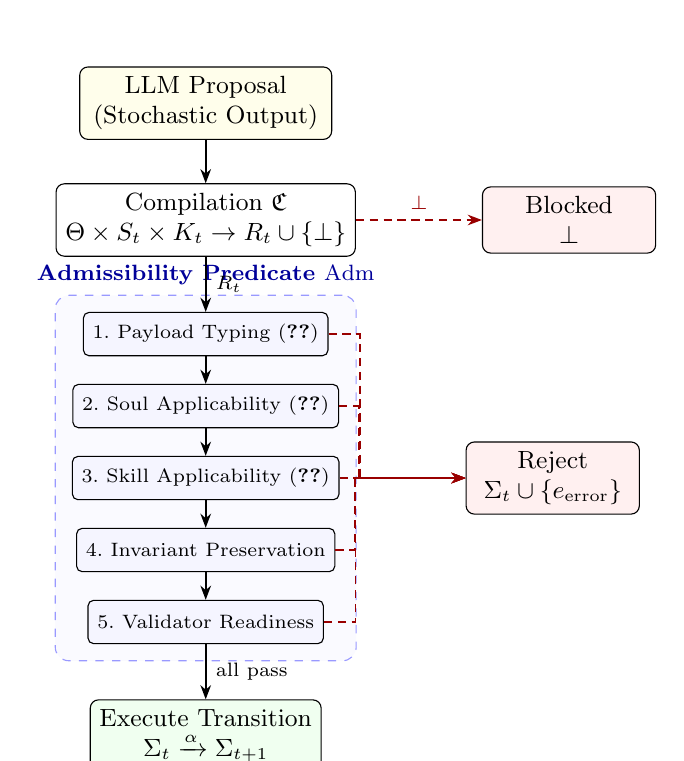
\begin{tikzpicture}[
  node distance=0.55cm and 0.8cm,
  block/.style={draw, rounded corners=3pt, minimum width=3.2cm, minimum height=0.7cm, align=center, font=\small, fill=white},
  decision/.style={draw, diamond, aspect=2.2, inner sep=1pt, align=center, font=\small, fill=white},
  reject/.style={draw, rounded corners=3pt, minimum width=2.2cm, minimum height=0.6cm, align=center, font=\small, fill=red!6},
  accept/.style={draw, rounded corners=3pt, minimum width=2.8cm, minimum height=0.6cm, align=center, font=\small, fill=green!6},
  check/.style={draw, rounded corners=2pt, minimum width=2.6cm, minimum height=0.55cm, align=center, font=\scriptsize, fill=blue!4},
  arr/.style={-{Stealth[length=1.8mm]}, semithick},
  darr/.style={-{Stealth[length=1.8mm]}, semithick, densely dashed, red!60!black}
]
  \node[block, fill=yellow!8] (llm) {LLM Proposal\\(Stochastic Output)};
  \node[block, below=of llm] (comp) {Compilation $\mathfrak{C}$\\$\Theta \times S_t \times K_t \to R_t \cup \{\bot\}$};
  \draw[arr] (llm) -- (comp);

  \node[reject, right=1.6cm of comp] (cfail) {Blocked\\$\bot$};
  \draw[darr] (comp) -- node[above,font=\scriptsize]{$\bot$} (cfail);

  \node[check, below=0.7cm of comp] (t1) {1.~Payload Typing (\cref{ax:payload-typing})};
  \node[check, below=0.35cm of t1] (t2) {2.~Soul Applicability (\cref{ax:soul-applicability})};
  \node[check, below=0.35cm of t2] (t3) {3.~Skill Applicability (\cref{ax:skill-applicability})};
  \node[check, below=0.35cm of t3] (t4) {4.~Invariant Preservation};
  \node[check, below=0.35cm of t4] (t5) {5.~Validator Readiness};
  \draw[arr] (comp) -- node[right,font=\scriptsize]{$R_t$} (t1);
  \draw[arr] (t1) -- (t2);
  \draw[arr] (t2) -- (t3);
  \draw[arr] (t3) -- (t4);
  \draw[arr] (t4) -- (t5);

  \node[reject, right=1.6cm of t3] (rej) {Reject\\$\Sigma_t \cup \{e_{\mathrm{error}}\}$};
  \draw[darr] (t1.east) -- ++(0.4,0) |- (rej);
  \draw[darr] (t2.east) -- ++(0.25,0) |- (rej);
  \draw[darr] (t3) -- (rej);
  \draw[darr] (t4.east) -- ++(0.25,0) |- (rej);
  \draw[darr] (t5.east) -- ++(0.4,0) |- (rej);

  \node[accept, below=0.7cm of t5] (exec) {Execute Transition\\$\Sigma_t \xrightarrow{\alpha} \Sigma_{t+1}$};
  \draw[arr] (t5) -- node[right,font=\scriptsize]{all pass} (exec);

  % Zone label
  \begin{scope}[on background layer]
    \node[draw=blue!40, dashed, rounded corners=5pt, fill=blue!2,
          fit=(t1)(t2)(t3)(t4)(t5), inner sep=6pt,
          label={[font=\footnotesize\bfseries, text=blue!60!black]above:Admissibility Predicate $\Adm$}] {};
  \end{scope}
\end{tikzpicture}
\caption{Instruction reserve flow.  The LLM proposes a typed reserve candidate; the compilation map~$\mathfrak{C}$ rejects malformed proposals as~$\bot$.  Compiled reserves pass through the five-conjunct admissibility predicate.  Failure at any conjunct blocks the transition; only fully admissible reserves enable state mutation.}
\label{fig:reserve-flow}
\end{figure}

\newpage
\section{Node Micro-Architecture}

The \AOC{} micro-architecture models agentic execution as typed graph composition. The formal claim in this section is limited: node-level behavior is represented compositionally, and feedback is admitted only through an explicitly guarded construction.

\begin{definition}[Primitive Basis $\mathsf{Gen}$]
We define a fixed generator set $\mathsf{Gen}$ of atomic protocol primitives from which legal node terms are built:
\[
\mathsf{Gen}=\{\mathsf{Observe},\mathsf{Generate},\mathsf{Verify},\mathsf{Compress},\mathsf{Route},\mathsf{Commit},\mathsf{Correct},\mathsf{ToolIntent},\mathsf{ToolJoin}\}.
\]
The neuromorphic extension track (\cref{sec:neuromorphic-extension}) interprets instances of these primitives as abstract hardware events; it does not identify $\mathsf{Gen}$ with any specific silicon instruction set.
\end{definition}

\begin{center}
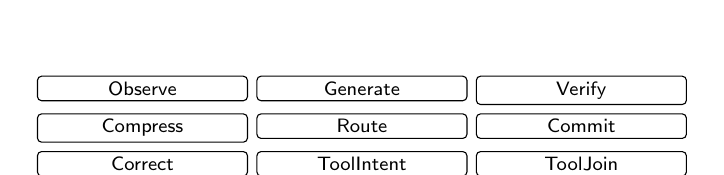
\begin{tikzpicture}
\matrix (M) [matrix of math nodes, column sep=3pt, row sep=3pt, every node/.append style={gencell}] {
\mathsf{Observe} & \mathsf{Generate} & \mathsf{Verify} \\
\mathsf{Compress} & \mathsf{Route} & \mathsf{Commit} \\
\mathsf{Correct} & \mathsf{ToolIntent} & \mathsf{ToolJoin} \\
};
\end{tikzpicture}
\end{center}

\subsection{Categorical Semantics}

\begin{definition}[Node Term]
A node term \(N\) is a well-typed morphism in the free strict symmetric monoidal category generated by \(\mathsf{Gen}\). Serial composition, tensor, identities, and symmetries are inherited from that free construction.
\end{definition}

\begin{definition}[Guarded Trace]\label{def:guarded-trace}
Let \(f:A\otimes M\to B\otimes M\) be a well-typed morphism. A guarded trace
\[
\mathrm{Tr}^{g}_{M}(f):A\to B
\]
is admissible only if the feedback carrier \(M\) passes through a verification or routing stage before re-entry and there exists a well-founded ranking map \(\varpi_f\) on the \(M\)-state such that each feedback cycle strictly decreases \(\varpi_f\) or strictly decreases one of the global bounds \(b,d,N\). Thus guarded trace is a partial feedback constructor on legal node terms, not an unrestricted trace on the whole category.
\end{definition}

\paragraph{Why SMC structure is enough here.}
The SMC layer supplies only the compositional syntax needed for serial and parallel wiring. Resource sensitivity is enforced by the typing discipline together with the guarded-trace side condition, rather than by any claim that arbitrary copying or arbitrary recursion is available.

\subsection{Node Denotation and State Transformation}

\begin{definition}[Node Denotation]
A node denotation is a typed state transformer mapping inputs to a probability distribution (or power set) of output states:
\[
\llbracket N \rrbracket : X_N \times \mathcal{I}(N) \to \mathcal{P}(X_N \times \mathcal{O}(N)).
\]
\end{definition}

\paragraph{Relation to the asynchronous substrate.}
This denotation is the interface later used in the restricted mapping to the event-driven substrate. In that mapping, a generator such as \(\mathsf{Generate}\) corresponds to a higher-cost event source, while \(\mathsf{Verify}\) and \(\mathsf{Route}\) correspond to lower-cost control transitions that may suppress further expansion.

\begin{lemma}[Closure under Typed Composition]\label{lem:closure-typed-composition}
Assume:
\begin{enumerate}
\item every primitive generator \(g \in \mathsf{Gen}\) is well-typed;
\item every primitive generator preserves the invariant \(I\);
\item the trace operator is only applied under the guardedness condition stated in \cref{def:guarded-trace};
\item guarded trace does not violate the global bounds \(b,d,N\).
\end{enumerate}
Then the class of legal node terms is closed under the constructors generated by \(\mathsf{Gen}\), tensor, composition, and guarded trace. In particular, every such composite term is well-typed and preserves \(I\).
\end{lemma}

\begin{proof}
We argue by structural induction on legal term formation.

For primitive terms, the claim is exactly assumptions (1) and (2).

For tensor and composition, well-typedness follows from the structural rules of the ambient symmetric monoidal category. Since \(I\) is preserved by each component and the typing rules only permit compositions along matching interfaces, the composite again preserves \(I\).

For guarded trace, assumption (3) ensures that trace is only formed when the feedback channel satisfies the required guardedness side-condition. By the typing rule for guarded trace, the resulting term is well-typed. By assumption (4), the trace step does not exceed the prescribed bounds \(b,d,N\), so legality is preserved. Since the traced subterm preserves \(I\) and the guarded feedback does not introduce any new unverified behavior outside the traced interface, the resulting term also preserves \(I\).

Hence every legal composite term is well-typed and invariant-preserving.
\end{proof}

\begin{theorem}[Node Composition Closure]
The class of legal nodes is closed under identities, serial composition, parallel composition, symmetry, and guarded feedback.
\end{theorem}

\begin{proof}[Proof sketch]
This follows from \cref{lem:closure-typed-composition} together with the freeness of the symmetric monoidal category generated by \(\mathsf{Gen}\).
\end{proof}
\newpage
\section{Global GoT Topology}

\begin{definition}[Global Typed GoT Graph]
A global graph is
\[
G=(V,E,s,t,\tau_V,\tau_E,\mathsf{node},\mathsf{chan}),
\]
where \(\mathsf{node}(v)\) is a legal node term and \(\mathsf{chan}(e)\) carries channel metadata.
\end{definition}

\begin{definition}[Compatibility Constraint]
For each edge \(e:u\to v\),
\[
\mathcal{O}(\mathsf{node}(u)) \models \tau_E(e) \models \mathcal{I}(\mathsf{node}(v)).
\]
\end{definition}

\begin{definition}[Typed Rewrite Operations]
Admissible graph operations include
\[
\mathsf{Expand},\quad \mathsf{Merge},\quad \mathsf{Prune},\quad \mathsf{Feedback}.
\]
\end{definition}

\begin{theorem}[Graph Rewrite Preservation]\label{thm:graph-rewrite-preservation}
Let \(G\) be a globally typed graph.
\begin{enumerate}
    \item \(\mathsf{Expand}\) preserves global typing provided every newly introduced node term is legal and every newly introduced edge satisfies the compatibility constraint.
    \item \(\mathsf{Prune}\) preserves global typing provided it removes only a node together with all incident edges, or more generally a subgraph whose deletion leaves all remaining edges unchanged.
    \item \(\mathsf{Feedback}\) preserves global typing provided the feedback edge satisfies the guarded compatibility condition.
    \item \(\mathsf{Merge}\) preserves global typing provided there exists a merge-policy witness certifying interface compatibility, certificate reconciliation, and preservation of any required invariants.
\end{enumerate}
\end{theorem}

\begin{proof}
We verify each rewrite separately.

For \(\mathsf{Expand}\), all pre-existing nodes and edges retain their original typings. By hypothesis, each newly added node is a legal node term, and each newly added edge \(e:u \to v\) satisfies
\[
\mathcal{O}(\mathsf{node}(u)) \models \tau_E(e) \models \mathcal{I}(\mathsf{node}(v)).
\]
Hence the expanded graph satisfies the global typing condition.

For \(\mathsf{Prune}\), the operation deletes nodes and/or edges but does not modify the typing data of any remaining node or remaining edge. Therefore every compatibility judgment that held before pruning still holds in the residual graph. Thus the residual graph remains globally typed.

For guarded \(\mathsf{Feedback}\), the only new obligation is the compatibility of the feedback connection. By the guarded compatibility side-condition, the new feedback edge is well-typed; all other typing judgments are unchanged. Hence global typing is preserved.

For \(\mathsf{Merge}\), the merged node may identify two or more prior interfaces. Global typing is preserved only if the merge-policy witness certifies that the resulting node has a legal interface type, that incoming and outgoing edges remain compatible with that interface, and that any required certificates or invariants are correctly transported to the merged configuration. Under exactly those witness conditions, the rewritten graph is globally typed.
\end{proof}

\section{Constraint and Policy Layer}

\subsection[Soul-Constrained Subagents and Skills]{Soul-Constrained Subagents and Repository-Native Skills}\label{sec:soul-skills}

This section refines the role of the soul and skill layers without changing the axioms introduced in \cref{ax:payload-typing,ax:soul-applicability,ax:skill-applicability}. The purpose here is to describe the runtime objects that realize those predicates.

\begin{remark}[Meaning of ``soul'' in this paper]\label{rem:soul-meaning}
The term \emph{soul} denotes a fixed, runtime policy envelope that encodes role, expertise boundaries, epistemic policy, permitted and prohibited behaviors, output discipline, declared human-in-the-loop approval patterns, and an identity handle.
It persists across turns and sessions; it is not rewritten by transient context.
The word is an architectural metaphor---it carries no metaphysical, theological, or consciousness-related connotation.
In formal terms, the soul is a conjunctive predicate that must be satisfied for any reserve node to pass the admissibility check (\cref{ax:soul-applicability}).
\end{remark}

\begin{definition}[Operational Soul]
An operational soul is a runtime constraint object
\[
S_t=(\rho_t,\epsilon_t,\Gamma_t,\Pi_t,\Psi_t,\Omega_t,\Upsilon_t),
\]
where:
\begin{center}
\small
\begin{tabular}{@{}p{0.16\linewidth}>{\raggedright\arraybackslash}p{0.76\linewidth}@{}}
\toprule
\textbf{Component} & \textbf{Role} \\
\midrule
\(\rho_t\) & role and expertise boundary \\
\(\epsilon_t\) & epistemic policy, including uncertainty and abstention behavior \\
\(\Gamma_t\) & allowed reasoning and response modes \\
\(\Pi_t\) & permission envelope for tools, files, and side effects \\
\(\Psi_t\) & prohibited behaviors and refusal conditions \\
\(\Omega_t\) & output discipline and contract obligations \\
\(\Upsilon_t\) & stable identity or attestation handle \\
\bottomrule
\end{tabular}
\end{center}
\end{definition}

\begin{definition}[Soul-Constrained Admissibility]
A reserve node is executable only if
\[
\Adm(r_i \mid P,S_t,K_t,I,\Sigma_t)=1,
\]
where admissibility includes soul compatibility as one of its conjunctive checks.
\end{definition}

\begin{definition}[Repository-Native Skill]
A repository-native skill is a runtime capability represented jointly by executable logic, an explicit contract document, a repository location and loading convention, and any local assets or tests needed for reliable invocation.
\end{definition}

\begin{definition}[Skill Contract Document]
A \texttt{SKILL.md} document is the human- and model-readable contract associated with a skill. At minimum it specifies purpose, trigger conditions, required inputs, expected outputs, preconditions, postconditions, safety constraints, and environment assumptions.
\end{definition}

\begin{definition}[Free-Copy Contract]
If \(C_k\) is the authoritative contract of skill \(k\), a free-copy \(\widetilde{C}_k\) is a read-optimized representation satisfying
\[
\mathrm{Sem}(\widetilde{C}_k)=\mathrm{Sem}(C_k)
\]
for the invocation-relevant clauses, while omitting implementation details unnecessary for planning.
A free-copy excludes heavy assets (source code, test fixtures, binary dependencies) so that the planner can compare and route across many skills without loading full implementations into context.
\end{definition}

\begin{lemma}[Soul-Gated Exclusion]
If admissibility is filtered through soul constraints before execution, then every executed reserve action satisfies the soul predicate by construction.
\end{lemma}

\begin{proof}
An action is executable only if
\[
\Adm(r_i \mid P,S_t,K_t,I,\Sigma_t)=1.
\]
By definition of admissibility, soul compatibility is a necessary conjunct. Hence any executed reserve action satisfies \(\Soul(r_i,S_t)=1\).
\end{proof}

\begin{lemma}[Skill Composability]
Suppose each skill is specified by executable logic together with an explicit pre/postcondition contract. Then skill invocation is testable against its contract and composable whenever the postcondition of one skill entails the precondition of the next.
\end{lemma}

\begin{proof}
Testability follows because the contract determines a concrete validation criterion for each invocation outcome. Composability follows from standard contract composition: if skill \(S_1\) establishes \(Q\) and skill \(S_2\) requires \(P\) with \(Q \Rightarrow P\), then the sequential composition \(S_2 \circ S_1\) is well-formed.
\end{proof}

\subsection{Routing and Dual-Lane Qwen Policy}\label{sec:routing-policy}

\begin{definition}[Routing Action]
A routing action is
\[
u_t=(v_t,\alpha_t,\ell_t,\tau_t),
\]
where \(v_t\) is the next focal node, \(\alpha_t\) the next transition class, \(\ell_t\in\{\fast,\deep,\mixed\}\) the model lane, and \(\tau_t\) an optional tool target.
\end{definition}

\begin{definition}[Routing Objective]
For admissible action \(u\), define
\[
J_t(u)=\alpha\,\widehat{Q}_t(u)-\beta\,\widehat{C}_t(u)-\gamma\,\widehat{R}_t(u)+\delta\,\widehat{V}_t(u),
\]
where \(\widehat{Q}_t\) estimates output quality, \(\widehat{C}_t\) estimates latency or energy cost, \(\widehat{R}_t\) estimates validation or policy risk, and \(\widehat{V}_t\) estimates verification utility.
\end{definition}

\begin{hypothesis}[Dual-Lane Doctrine]
A lane policy that reserves \(\fast\) for routing, lightweight continuation, and micro-planning, while reserving \(\deep\) for synthesis, code generation, and verification-heavy steps, may improve cost-latency-quality tradeoffs in local operation.
\end{hypothesis}

\begin{remark}[Concrete lane assignment]\label{rem:lane-assignment}
In the current reference implementation, the fast lane ($\fast$) is bound to \texttt{qwen3.5:4b} and the deep lane ($\deep$) is bound to \texttt{qwen3.5:9b}. This binding is an implementation choice rather than an empirical result: the smaller lane is used for low-cost control work such as routing and prompt compaction, while the larger lane is reserved for multi-step synthesis and verification-heavy reserve compilation. The $\mixed$ lane interleaves both models within a single execution trace under the routing objective \(J_t(u)\).
\end{remark}

\begin{lemma}[Fast-Lane Sufficiency]
If a candidate action requires no multi-hop tool use, no long-horizon synthesis, and low verification burden, then choosing \(\fast\) is admissible.
\end{lemma}

\begin{lemma}[Deep-Lane Escalation]
If a candidate action requires code generation, long-horizon synthesis, or high-risk tool selection, then \(\deep\) is admissible and preferred whenever \(J_t(\deep)>J_t(\fast)\).
\end{lemma}

\paragraph{Summary of the constraint layer.}
At this point the protocol has established three layers of control.
The \emph{core ontology} (\cref{ax:payload-typing,ax:soul-applicability,ax:skill-applicability}) fixes the predicates every reserve node must satisfy.
The \emph{constraint and policy layer} refines those predicates into runtime objects: soul states, skill contracts, free-copy contract summaries, and a dual-lane routing policy.
The following section assembles these into a global execution semantics that governs how the protocol transitions between states.

\section{Execution Semantics}\label{sec:execution-semantics}

This section composes the objects of \cref{sec:core-ontology} into a labeled transition system. \Cref{fig:reserve-flow} summarizes the proposal-to-execution pipeline; \cref{def:admissibility} is the formal statement of the admissibility gate.

\begin{definition}[Global Execution State]
At time \(t\), the global execution state is
\[
\Sigma_t=(G_t,U_t,X_t,C_t,R_t,\Pi_t,B_t,K_t,\mathcal{K}_t,S_t,A_t,Z_t),
\]
where the components are as follows:
\begin{center}
\small
\begin{tabular}{@{}p{0.14\linewidth}p{0.78\linewidth}@{}}
\toprule
\textbf{Symbol} & \textbf{Role} \\
\midrule
\(G_t\) & current graph \\
\(U_t\) & active frontier \\
\(X_t\) & node-local states \\
\(C_t\) & channel states \\
\(R_t\) & reserve \\
\(\Pi_t\) & provenance \\
\(B_t\) & budgets \\
\(K_t\) & active skill context \\
\(\mathcal{K}_t\) & certificates \\
\(S_t\) & soul \\
\(A_t\) & current artifact \\
\(Z_t\) & execution status \\
\bottomrule
\end{tabular}
\end{center}
\end{definition}

\begin{definition}[Admissibility Predicate]\label{def:admissibility}
For reserve element \(r\in R_t\),
\[
\Adm(r \mid P,S_t,K_t,I,\Sigma_t)\in\{0,1\}
\]
holds iff
\[
\begin{aligned}
\Adm(r \mid P,S_t,K_t,I,\Sigma_t)=1
\iff{}\;& \Type(r \mid P,K_t)=1 \\
&\land \Soul(r,S_t)=1 \\
&\land \Skill(r,K_t)=1 \\
&\land \mathrm{InvPres}(r \mid I,\Sigma_t)=1 \\
&\land \mathrm{Pre}(r \mid \Sigma_t,\mathcal{K}_t)=1.
\end{aligned}
\]
The first three conjuncts are exactly the applicability predicates fixed by \cref{ax:payload-typing,ax:soul-applicability,ax:skill-applicability}; the final two conjuncts capture invariant preservation and validator readiness in the current state.
\end{definition}

\begin{definition}[Legal Transition]
A labeled transition
\[
\Sigma_t \xrightarrow{\alpha} \Sigma_{t+1}
\]
is legal iff it is generated by a typed graph rewrite or reserve action whose enabling reserve node satisfies the admissibility predicate, whose required budgets remain available, and whose post-state is globally typed.
\end{definition}

\begin{definition}[Canonical Score]
For artifact \(A_t\), define
\[
\sigma(A_t,I,T)=\frac{1}{2}\SV(A_t,T)+\frac{1}{2}\IC(A_t,I).
\]
\end{definition}
In the current reference implementation, the canonical score is computed inside \texttt{aoc-api} and stored on \texttt{ControllerState.score}; it is persisted with selected artifacts and trace metadata.

\begin{definition}[Completion]
A state is complete iff a final artifact exists, required validator certificates exist, no required pending tool result remains unresolved, and bounded termination conditions permit exit.
\end{definition}

\begin{definition}[Typed Equivalence]
Two execution states are typed-equivalent if they differ only by renaming of fresh identifiers and by representation choices that preserve all typing, certificate, provenance, and budget-relevant data.
\end{definition}

\subsection{Operational Execution Model}\label{sec:operational-execution-model}

The formal transition system abstracts a concrete control loop already visible in the reference architecture. At the protocol level, a mediated turn follows a Reflect\(\to\)Propose\(\to\)Execute cycle; in the current reference implementation the Reflect phase is split across \texttt{aoc-api}, \texttt{nemoclaw}, and \texttt{general\_nemo}, while the Execute phase terminates at \texttt{arcade-mcp} or \texttt{nemo-executor} only after deterministic checks pass.

\paragraph{Reserve lifecycle.}
For a single reserve candidate \(r\), the lifecycle is:
\begin{enumerate}[leftmargin=1.5em]
    \item \textbf{Reflect.} \texttt{aoc-api} compiles the inbound request into \(P\), binds operator and session identity, and fixes the immutable \texttt{M0} run context; \texttt{general\_nemo} reconstructs persisted session state and optional \texttt{M2} correction memory, while branch-local deltas remain \texttt{M1} data.
    \item \textbf{Propose.} The active Qwen lane (\(\fast\), \(\deep\), or \(\mixed\)) produces a proposal-only turn result under the PromptCompiler and OODA budget profile. The current reference implementation may use a micro-lane probe or a fast-lane cascade before escalating to the deep lane.
    \item \textbf{Compile.} The reserve builder serializes tool intents and final text into a turn-local instruction reserve. In the current reference implementation this appears as the \texttt{instruction\_reserve} envelope returned by \texttt{general\_nemo}; at the protocol level, any equivalent typed representation is acceptable.
    \item \textbf{Classify.} Each candidate action is classified into one of three protocol tiers: \texttt{SAFE}, \texttt{APPROVAL\_REQUIRED}, or \texttt{FORBIDDEN}. In the current Rust executor these tiers are realized as permission modes \texttt{Allow}, \texttt{Prompt}, and \texttt{Deny}; the paper's tier names are therefore a protocol-level normalization rather than a claim about wire-level enum names.
    \item \textbf{Admit or block.} Payload typing, soul applicability, skill applicability, invariant preservation, validator readiness, and any approval requirement are checked at the reserve gate. A \texttt{FORBIDDEN} candidate or an unapproved \texttt{APPROVAL\_REQUIRED} candidate is blocked before side effects.
    \item \textbf{Execute.} Only an admitted candidate can reach \texttt{arcade-mcp} or \texttt{nemo-executor}. The tool broker must return a typed result or typed failure; it does not widen authority granted upstream.
    \item \textbf{Verify.} The gateway and verified scheduler update request-journal checks, step verification roots, and execution verification status. Follow-up verification may be polled through \texttt{/api/v1/executions/\{id\}/verification}; at the protocol level, commit remains contingent on the verification outcome rather than on tool success alone.
    \item \textbf{Provenance and commit.} Provenance is extended with reserve identifiers, artifact hashes, certificates, and verification roots. A commit is auditable only when the resulting trace is bound to \(\mathrm{Hash}(\Lambda)\).
\end{enumerate}

\paragraph{Approval and creator control.}
\texttt{APPROVAL\_REQUIRED} actions remain proposal-only until creator approval exists. In the current reference implementation, the control surfaces are the \texttt{pending\_action} envelope, the \texttt{tool\_confirmed} request flag, the session-scoped \texttt{/v1/feedback} loop, and the Jokuh owner binding carried via \texttt{owner\_user\_id}. The manuscript models these surfaces as an abstract approval token so that other implementations may persist approval state differently. Per-turn reserve construction, pending confirmation, and human feedback are implemented today; end-to-end reserve-mediated approval of every tool call across the full OODA loop remains an implementation obligation rather than a reported completion result.

\paragraph{Retry discipline, degraded mode, and resume behavior.}
Retries are bounded and consume fresh budget. The current reference implementation includes a safe elaboration retry for too-short answers, repair and compensation hooks in the typed action runtime, and degraded portal profiles that force read-only behavior (\texttt{degraded\_read\_only=true}, \texttt{allow\_side\_effects=false}) when full capability surfaces are unavailable. After restart, Nemoclaw resumes session state from persisted JSON and correction memory from \texttt{corrections.jsonl}; traces and verification state remain queryable through the gateway. This is restart recovery, not a claim of distributed consensus or exactly-once execution.

\begin{theorem}[Boundedness]\label{thm:boundedness}
Assume:
\begin{enumerate}
    \item the initial graph \(G_0\) is finite;
    \item the initial reserve is finite;
    \item the budgets \(b,d,N\) are finite;
    \item every legal transition preserves global typing and does not increase the bounded resource vector
    \[
    \mu(\Sigma_t):=\bigl(B_t^{\mathrm{branch}},\; B_t^{\mathrm{depth}},\; B_t^{\mathrm{budget}},\; |R_t|,\; |U_t|\bigr)
    \]
    in the lexicographic order, with at least one strictly decreasing component on every non-stuttering transition;
    \item the space of well-typed local states, channel states, certificates, and artifacts is finite up to typed equivalence.
\end{enumerate}
Then every execution trace is finite or eventually reaches a declared terminal state.
\end{theorem}

\begin{proof}
By assumption, every reachable state is well-typed. Because the initial graph, reserve, and budgets are finite, and because reachable local states, channel states, certificates, and artifacts range over only finitely many equivalence classes, the set of reachable states is finite up to typed equivalence.

Now consider any execution trace. If infinitely many non-stuttering transitions occurred, assumption (4) would produce an infinite descending chain in the well-founded lexicographic order on \(\mu\), which is impossible. Therefore only finitely many non-stuttering transitions can occur.

Hence every infinite trace must eventually stutter within a finite equivalence class of states. By the operational convention that such a situation is represented by a declared terminal status (success, failure, or deadlock), the execution is finite or enters a terminal state.
\end{proof}

\begin{proposition}[Decidability of Next-Step Legality]\label{prop:decidable-next-step}
For any nonterminal state \(\Sigma_t\), it is decidable whether there exists a legal outgoing transition. Consequently, every nonterminal state is either enabled (a legal transition exists) or deadlocked (none exists).
\end{proposition}

\begin{proof}
By definition, the active frontier \(U_t\) and reserve \(R_t\) are finite in every reachable state. The legality of each candidate transition is determined by finitely many checks: typing compatibility, admissibility, budget availability, validator preconditions, and any rewrite-specific side conditions. Each of these checks is decidable by finite inspection of the current state. Therefore the set of legal outgoing transitions is computable, and in particular it is decidable whether it is empty. If it is nonempty, the state is enabled; otherwise it is deadlocked.
\end{proof}

\subsection{Failure and Recovery Semantics}\label{sec:failure-recovery}

Failure handling in \AOC{} is part of the protocol envelope, not an implementation afterthought. The governing rule is that failure does not create authority: a failed proposal, failed validation, or failed side effect yields a typed artifact and an auditable trace entry, but it does not silently advance the state machine.

\begin{table}[H]
\centering
\caption{Failure and recovery semantics.}
\label{tab:failure-recovery}
\footnotesize
\begin{tabularx}{\linewidth}{@{}>{\raggedright\arraybackslash}p{0.22\linewidth}>{\raggedright\arraybackslash}p{0.17\linewidth}X>{\raggedright\arraybackslash}p{0.23\linewidth}@{}}
\toprule
\textbf{Failure class} & \textbf{Stop point} & \textbf{Artifact emitted} & \textbf{Retry / recovery rule} \\
\midrule
Reserve compilation failure & Reserve builder / \(\mathfrak{C}\) & Compile rejection plus \texttt{VerifiedFailure} with schema or contract rationale; request-journal event & Retry only as a new proposal; the rejected node never acquires execution authority \\
\addlinespace
Admissibility failure & Reserve gate & Rejected reserve record with failed conjuncts and provenance pointer & Retry requires a changed reserve, changed state, or new approval evidence; no mutation occurs before that \\
\addlinespace
Tool invocation failure & Tool broker / executor & \texttt{TypedToolResult\{status=error\}} or \texttt{VerifiedFailure\{side\_effect\}}; rollback or compensation event if applicable & Retry is allowed only as a fresh reserve and only after compensation or explicit operator policy if side effects may have occurred \\
\addlinespace
Missing or contradictory validator output & Verification or commit gate & \texttt{verification\_status=failed}, failed certificates, no commit signature & Automatic promotion stops; follow-up verification or human/operator intervention is required before reattempt \\
\addlinespace
Approval absent & Approval gate & \texttt{ApprovalRequest} or \texttt{pending\_action} artifact; trace remains open and auditable & Wait for creator approval; no autonomous escalation from \texttt{APPROVAL\_REQUIRED} to executable \\
\addlinespace
Stuck execution, deadlock, or budget exhaustion & Scheduler / controller & \texttt{VerifiedFailure\{deadlock\}} or \texttt{VerifiedFailure\{budget\}} & Requires a new execution with revised budget, revised problem compilation, or operator intervention \\
\addlinespace
Restart or interruption & Startup recovery boundary & Recovery event plus retained session, trace, and verification metadata & Reload persisted session and correction memory; treat any in-flight external action as unverified until re-polled or rerun \\
\addlinespace
Degraded mode entry & Routing boundary & Degraded-execution record, narrowed tool policy, no side-effect admission & Remain read-only or low-authority until health and release checks pass; degraded mode is a narrower protocol path, not equivalence with full mode \\
\bottomrule
\end{tabularx}
\end{table}

\paragraph{Rollback, logging, and audit rules.}
Compilation and admissibility failures occur before mutation and therefore require no rollback of persistent skill or graph state. Side-effecting execution failures may require compensation under \(\rho\); in the current reference implementation the typed action runtime records compensation attempts and rollback outcomes, while the bounded controller rolls back non-winning branches before commit. When an execution resumes after interruption, previously persisted session state, correction memory, request-journal entries, and execution verification metadata may be reloaded, but any in-flight external action is treated as unverified until follow-up verification succeeds or an operator explicitly restarts it. The trace remains auditable even when the run fails because the failure artifact, failed checks, and release identity remain part of the same provenance chain.

\section{Authority and Deployment Truth}

\subsection{Runtime Authority}\label{sec:runtime-authority}

Runtime authority in \AOC{} is intentionally non-uniform. Proposal generation, reserve compilation, tool brokering, side-effect execution, and release verification occur in different components because they carry different trust assumptions. The point of the layering is to move authority into deterministic control surfaces and to leave stochastic models in a proposal-only role.

\begin{center}
\small
\begin{tabularx}{\linewidth}{@{}>{\raggedright\arraybackslash}p{0.20\linewidth}>{\raggedright\arraybackslash}p{0.28\linewidth}X@{}}
\toprule
\textnormal{\textbf{Component}} & \textnormal{\textbf{Authority Held}} & \textnormal{\textbf{Verification Obligation / Limitation}} \\
\midrule
\texttt{aoc-api} & request admission, identity binding, reserve gating, trace emission & compiles problem specifications, checks permissions, and may authorize or reject a transition; it does not execute the model's proposal directly \\
\texttt{nemoclaw} & bounded orchestration and frontier management & schedules model-facing work and transition order under policy; it cannot bypass reserve admissibility or release checks \\
\texttt{general\_nemo} & session and prompt-state maintenance & maintains conversational state, compaction, and prompt formatting; it does not grant tool, commit, or deployment authority \\
\texttt{arcade-mcp} and \texttt{nemo-executor} & tool brokering and local side effects & execute only approved actions, return typed tool results, and emit execution evidence; they are not permitted to widen authority received from upstream layers \\
\texttt{ollama} & local inference serving & hosts open-weight models and returns proposals; it does not own commit, permission, or attestation logic \\
Qwen-family model lanes & stochastic proposal generation & generate reserve candidates for control and synthesis tasks; they may be informative or useful, but they are never self-authorizing \\
\bottomrule
\end{tabularx}
\end{center}

\Cref{fig:runtime-layers} summarizes the same layering: proposals flow upward from the inference substrate into the reserve gate and downward toward tools only after runtime approval. The model can influence what is proposed; it cannot, by protocol definition, decide that a proposal is admissible.

% --- FIGURE: Runtime Layering ---
% mermaid source: wp/diagrams/runtime-layers.mmd
\begin{figure}[H]
\centering
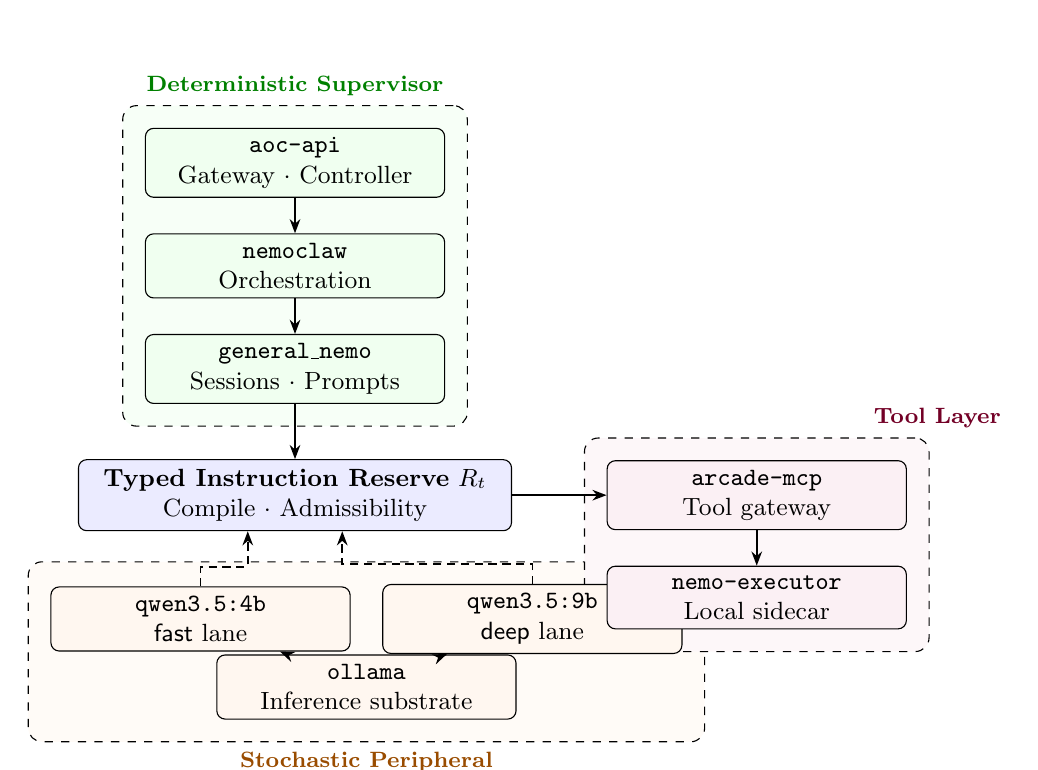
\begin{tikzpicture}[
  node distance=0.45cm and 1.2cm,
  comp/.style={draw, rounded corners=3pt, minimum width=3.8cm, minimum height=0.65cm, align=center, font=\small, fill=white},
  zone/.style={draw, dashed, rounded corners=5pt, inner sep=8pt},
  arr/.style={-{Stealth[length=1.8mm]}, semithick},
  warr/.style={-{Stealth[length=1.8mm]}, semithick, densely dashed}
]
  % Deterministic supervisor
  \node[comp, fill=green!6] (api) {\texttt{aoc-api}\\Gateway $\cdot$ Controller};
  \node[comp, fill=green!6, below=of api] (nc) {\texttt{nemoclaw}\\Orchestration};
  \node[comp, fill=green!6, below=of nc] (gn) {\texttt{general\_nemo}\\Sessions $\cdot$ Prompts};

  % Typed reserve boundary
  \node[comp, fill=blue!8, below=0.7cm of gn, minimum width=5.5cm] (res) {\textbf{Typed Instruction Reserve}~$R_t$\\Compile $\cdot$ Admissibility};

  % Stochastic peripheral
  \node[comp, fill=orange!6, below=0.7cm of res, xshift=-1.2cm] (qf) {\texttt{qwen3.5:4b}\\$\fast$ lane};
  \node[comp, fill=orange!6, right=0.4cm of qf] (qd) {\texttt{qwen3.5:9b}\\$\deep$ lane};
  \node[comp, fill=orange!6, below=of $(qf)!0.5!(qd)$] (oll) {\texttt{ollama}\\Inference substrate};

  % Tool layer
  \node[comp, fill=purple!6, right=1.2cm of res] (arc) {\texttt{arcade-mcp}\\Tool gateway};
  \node[comp, fill=purple!6, below=of arc] (ne) {\texttt{nemo-executor}\\Local sidecar};

  % Arrows
  \draw[arr] (api) -- (nc);
  \draw[arr] (nc) -- (gn);
  \draw[arr] (gn) -- (res);
  \draw[arr] (oll) -- (qf);
  \draw[arr] (oll) -- (qd);
  \draw[warr] (qf.north) -- ++(0,0.25) -| ([xshift=-0.6cm]res.south);
  \draw[warr] (qd.north) -- ++(0,0.25) -| ([xshift=0.6cm]res.south);
  \draw[arr] (res) -- (arc);
  \draw[arr] (arc) -- (ne);

  % Zone backgrounds
  \begin{scope}[on background layer]
    \node[zone, fill=green!3, label={[font=\footnotesize\bfseries,text=green!50!black]above:Deterministic Supervisor},
          fit=(api)(nc)(gn)] {};
    \node[zone, fill=orange!3, label={[font=\footnotesize\bfseries,text=orange!60!black]below:Stochastic Peripheral},
          fit=(qf)(qd)(oll)] {};
    \node[zone, fill=purple!3, label={[font=\footnotesize\bfseries,text=purple!60!black]above right:Tool Layer},
          fit=(arc)(ne)] {};
  \end{scope}
\end{tikzpicture}
\caption{Runtime layering.  The deterministic supervisor (green) compiles requests and governs execution.  Model proposals pass through the typed instruction reserve (blue) before reaching the tool layer (purple).  The stochastic peripheral (orange) generates candidates but never directly mutates system state.  Dashed arrows indicate proposal flow from model to reserve.}
\label{fig:runtime-layers}
\end{figure}

\paragraph{Trust boundary and failure surface.}
\Cref{tab:trust-boundary} makes explicit which layer is trusted for which kind of authority and which risks remain outside the stated guarantee envelope.

\begin{table}[H]
\centering
\caption{Trust boundary and failure surface map.}
\label{tab:trust-boundary}
\scriptsize
\begin{tabularx}{\linewidth}{@{}>{\raggedright\arraybackslash}p{0.16\linewidth}>{\raggedright\arraybackslash}p{0.11\linewidth}>{\raggedright\arraybackslash}p{0.14\linewidth}>{\raggedright\arraybackslash}p{0.14\linewidth}XX@{}}
\toprule
\textbf{Layer / surface} & \textbf{Trust status} & \textbf{Authority held} & \textbf{Primary risk} & \textbf{What the protocol checks} & \textbf{What remains outside the guarantee} \\
\midrule
User content / inbound request surface & Untrusted input & Can request work, not authorize mutation & Prompt injection, malformed payloads, ambiguous intent & Auth, input validation, problem compilation, request journaling & Semantic truth of user intent, compromised client endpoints \\
\addlinespace
Stochastic proposal layer (\texttt{ollama}, Qwen lanes) & Proposal-only & Suggests reserves, tool intents, and text & Hallucinated or unsafe proposals & Schema checks, reserve compilation, bounded budgets, admissibility re-check & Semantic correctness, hidden model defects, model-side leakage outside controlled deployment \\
\addlinespace
Typed reserve / admissibility layer & Deterministic control surface & Blocks or admits execution & Compiler bug, bypass, incorrect typing & Payload typing, soul, skill, invariants, validator readiness, approval state & Soundness depends on faithful implementation and validator coverage \\
\addlinespace
Deterministic controller / scheduler & High-trust runtime & Selects legal transitions, budget use, commit candidate & Ranking bug, starvation, undeclared heuristics & Boundedness, transition legality, step verification, trace updates & Policy bugs if code drifts from the published contract \\
\addlinespace
Skill registry / contract loader & Configuration trust & Resolves invocations to active contracts & Stale contracts, wrong side-effect class, capability mismatch & Active-contract resolution, schema checks, capability tags, preconditions & Malicious or incorrect skill code inside a declared contract surface \\
\addlinespace
Tool broker & Partial-trust bridge & Dispatches approved actions only & Tool injection, schema mismatch, hidden nested models & Approved-action check, typed result envelope, degraded read-only mode & Remote tool semantics, nested stochastic components, provider retention \\
\addlinespace
Local executor & Host-trust boundary & Performs local side effects & Filesystem or process mutation, permission bypass & Permission policy, interactive approval, typed success or failure, compensation hooks & Host compromise, kernel escape, incorrect side-effect classification \\
\addlinespace
External tools / remote APIs & External / untrusted & Own remote state and retention & Non-idempotence, opaque logging, provider-side policy drift & Contract wrappers, follow-up verification, provenance attribution & Provider behavior, legal process to provider, opaque downstream processing \\
\addlinespace
Provenance / evidence layer & Audit-trust surface & Records trace, hashes, verification roots & Tampering, truncation, storage drift & Hash chaining, verification status, release binding, append-only journal semantics & Storage compromise without independent attestation or operator controls \\
\addlinespace
Deployment attestation / release verifier & Promotion-trust surface & Decides whether a trace is auditable for a release & Image drift, stale evidence, tuple mismatch & Runtime-contract checks, manifest hashes, staged boot proof, model identity & Business-task correctness, host compromise, legal conclusions beyond the evidence set \\
\bottomrule
\end{tabularx}
\end{table}

\begin{axiom}[Runtime Authority]\label{ax:runtime-authority}
The model proposes reserve candidates. The runtime alone authorizes execution.
\end{axiom}

\subsection{Deployment Truth and Release Tuple}\label{sec:deployment-truth}

We treat deployment identity as part of the protocol semantics rather than as a post hoc operational note. A promoted execution environment is not determined by model weights alone. It is determined by the coupled configuration under which traces are interpreted: contracts, policy objects, model artifacts, container lineage, topology, and release evidence. Without that coupling, an execution trace may still be operationally useful, but it is not protocol-complete evidence.

\begin{definition}[Release Tuple]
A release is a cryptographic snapshot represented by
\[
\Lambda=(\mathcal{C},\mathcal{M},\mathcal{I},\mathcal{D},\mathcal{E}),
\]
where:
\begin{itemize}
    \item \(\mathcal{C}\): corpus and version state, including soul and skill contracts;
    \item \(\mathcal{M}\): model artifact identity;
    \item \(\mathcal{I}\): image lineage for the bounded runtime services;
    \item \(\mathcal{D}\): deployment topology and routing bounds;
    \item \(\mathcal{E}\): staged evidence, including tests and verification logs.
\end{itemize}
\end{definition}
In the current reference implementation, \(\Lambda\) is realized by the release manifest, image digests, runtime-contract baseline, model-identity probes, and staged ledgers consumed by \texttt{verify\_protocol\_deploy.py}; other implementations may serialize the same tuple differently.

\begin{axiom}[Deployment Truth]\label{ax:deployment-truth}
A promoted release is not fully defined without artifact identity, image lineage, topology, and staged evidence. Without \(\Lambda\), an execution trace cannot be independently audited.
\end{axiom}

\paragraph{Attestation and Traceability.}
Let \(\mathrm{Hash}(\Lambda)\) be the Merkle root of the release tuple. A committed reserve is auditable only when it is tied to that release identity:
\[
\Commit(R_t) \implies \mathrm{VerifySignature}(R_t,\mathrm{Hash}(\Lambda)) = 1.
\]
This condition does not prove semantic correctness of the reserve by itself. It proves that the reserve was produced, checked, and committed under a specific released configuration, which is a narrower but operationally important claim.

\paragraph{Operator meaning of deployment truth.}
The release tuple gives operators a place to bind together what usually drifts independently: the skill corpus, soul contracts, model digests, runtime images, routing policy, and staged verification outputs. That binding supports at least three enterprise-facing uses. First, it turns audit questions into concrete reconciliation tasks over hashes, signatures, and logs. Second, it lets promotion policy block stateful execution when the running topology does not match the staged topology. Third, it keeps deployment disputes from collapsing into narrative claims about what system was ``really'' running; the tuple defines the object to which traces attach. None of those properties substitute for application-specific validation, but they materially reduce ambiguity at the release boundary.

% --- FIGURE: Release Tuple ---
% mermaid source: wp/diagrams/release-tuple.mmd
\begin{figure}[H]
\centering
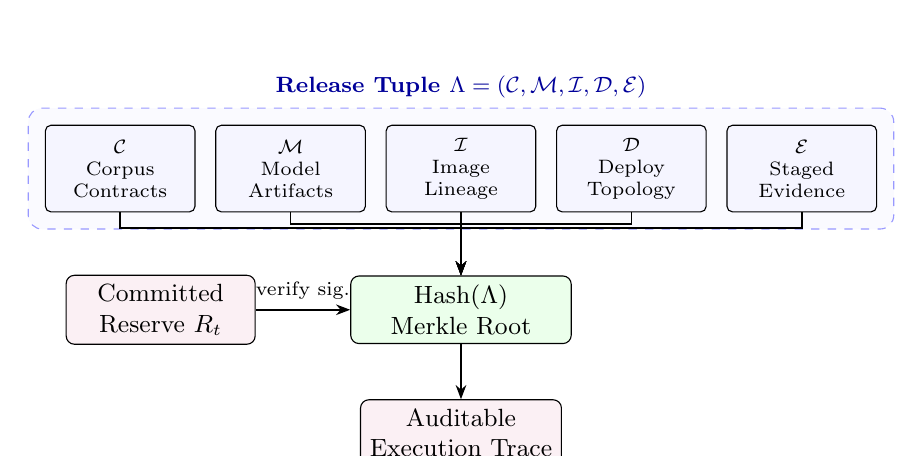
\begin{tikzpicture}[
  node distance=0.5cm and 0.25cm,
  comp/.style={draw, rounded corners=2pt, minimum width=1.9cm, minimum height=1.1cm, align=center, font=\scriptsize, fill=blue!4},
  hash/.style={draw, rounded corners=3pt, minimum width=2.8cm, minimum height=0.65cm, align=center, font=\small, fill=green!8},
  outbox/.style={draw, rounded corners=3pt, minimum width=2.4cm, minimum height=0.6cm, align=center, font=\small, fill=purple!6},
  arr/.style={-{Stealth[length=1.8mm]}, semithick}
]
  % Five components
  \node[comp] (c) {$\mathcal{C}$\\Corpus\\Contracts};
  \node[comp, right=of c] (m) {$\mathcal{M}$\\Model\\Artifacts};
  \node[comp, right=of m] (i) {$\mathcal{I}$\\Image\\Lineage};
  \node[comp, right=of i] (d) {$\mathcal{D}$\\Deploy\\Topology};
  \node[comp, right=of d] (e) {$\mathcal{E}$\\Staged\\Evidence};

  % Hash
  \node[hash, below=0.8cm of i] (h) {$\mathrm{Hash}(\Lambda)$\\Merkle Root};
  \draw[arr] (c.south) -- ++(0,-0.2) -| (h);
  \draw[arr] (m.south) -- ++(0,-0.15) -| (h);
  \draw[arr] (i) -- (h);
  \draw[arr] (d.south) -- ++(0,-0.15) -| (h);
  \draw[arr] (e.south) -- ++(0,-0.2) -| (h);

  % Committed reserve
  \node[outbox, left=1.2cm of h] (commit) {Committed\\Reserve $R_t$};
  \draw[arr] (commit) -- node[above,font=\scriptsize]{verify sig.} (h);

  % Audit output
  \node[outbox, below=0.7cm of h] (audit) {Auditable\\Execution Trace};
  \draw[arr] (h) -- (audit);

  % Lambda label
  \begin{scope}[on background layer]
    \node[draw=blue!40, dashed, rounded corners=5pt, fill=blue!2,
          fit=(c)(m)(i)(d)(e), inner sep=6pt,
          label={[font=\footnotesize\bfseries, text=blue!60!black]above:Release Tuple $\Lambda = (\mathcal{C},\mathcal{M},\mathcal{I},\mathcal{D},\mathcal{E})$}] {};
  \end{scope}
\end{tikzpicture}
\caption{Release tuple and deployment attestation.  The five components of~$\Lambda$ are hashed into a Merkle root.  A committed reserve is auditable only when its signature verifies against $\mathrm{Hash}(\Lambda)$, tying every execution trace to a specific released configuration.}
\label{fig:release-tuple}
\end{figure}

\section{Neuromorphic Extension Track}\label{sec:neuromorphic-extension}

This section studies a restricted mapping between the \AOC{} protocol's execution semantics and an abstract event-driven neuromorphic substrate.
The goal is not hardware equivalence in the general case; it is to state conditions (finite graph, finite reserve, guarded feedback, deterministic scheduler, bounded external delay) under which protocol transitions can be related to hardware event bundles via a weak bisimulation-style correspondence. No current \AOC{} runtime component computes this correspondence at execution time.
If such a mapping is instantiated, it would support event-driven implementations on neuromorphic hardware (e.g., Intel Loihi~2 \cite{intelloihi2}, IBM TrueNorth \cite{ibmtruenorth}) and would illustrate that typed protocol interfaces can, in principle, be preserved across substrates. The sketch below is not an implementation result.

\begin{definition}[Neuromorphic Substrate State]
An abstract substrate state is
\[
H_t=(\mathcal{C}^{\mathrm{hw}}_t,\mathcal{N}_t,\mathcal{W}_t,\mathcal{R}^{\mathrm{hw}}_t,\mathcal{Q}^{\mathrm{hw}}_t,\Xi_t),
\]
where \(\mathcal{C}^{\mathrm{hw}}_t\) are core states, \(\mathcal{N}_t\) neuron states, \(\mathcal{W}_t\) synapse states, \(\mathcal{R}^{\mathrm{hw}}_t\) router states, \(\mathcal{Q}^{\mathrm{hw}}_t\) event queues, and \(\Xi_t\) hardware cost counters.
\end{definition}
This object is conceptual and implementation-defined; the current reference implementation has no runtime object with this exact shape.

\begin{definition}[Event Packet]
An event packet is
\[
e=(a,t,p),
\]
where \(a\) is an address or route token, \(t\) a timestamp or logical order, and \(p\) a payload.
\end{definition}

\begin{definition}[LIF Dynamics]
For neuron \(j\), a simple leaky integrate-and-fire dynamic is
\[
\tau^{(j)}_m \frac{dv_j}{dt}=-(v_j-v^{(j)}_{\mathrm{rest}})+R_j I_j(t),
\]
with spike emission when \(v_j\ge v^{(j)}_{\mathrm{th}}\) and reset \(v_j\leftarrow v^{(j)}_{\mathrm{reset}}\).
\end{definition}

\begin{theorem}[Restricted Silicon Correspondence (conditional sketch)]
Subject to the restrictions above, one can define maps \(\Phi\) (protocol state to abstract substrate state) and \(\Psi\) (observable protocol labels to observable hardware bundles) such that pairs \((\Phi,\Psi)\) satisfy the usual weak bisimulation clauses on the restricted fragment.
\end{theorem}

\begin{proof}[Proof sketch]
Define \(\Phi\) by assigning legal node terms to disjoint substrate subnetworks, channel types to routing classes, and reserve-handling steps to guarded hardware transitions. Define \(\Psi\) on externally visible labels only. One then checks that each legal protocol step can be matched by a finite hardware microtrace (and conversely for hardware-observable steps in the fragment), abstracting internal silent steps. The maps \((\Phi,\Psi)\) are protocol-level correspondences only; the current reference implementation does not compute or persist them.
\end{proof}

\begin{remark}
The statement is intentionally limited to a finite, deterministic fragment. It does not assert bisimulation for the full deployed \AOC{} runtime or for arbitrary tool and network timing.
\end{remark}

\section[Learning and Adaptation]{Learning and Adaptation under Constraints}

Adaptation is subordinate to the protocol envelope, not the reverse. In this paper, learnable components may tune routing thresholds, prompt compaction heuristics, validator ordering, or other bounded controller parameters. They do not silently enlarge tool permissions, rewrite soul constraints, or alter release identity without a new released configuration. In the current reference implementation, the tunable surfaces most directly reflected in code are routing profile choice, session-compaction policy, validator ordering, and bounded tool-loop heuristics; the manuscript models a broader constrained-update family at protocol level and does not report live online learning in production.

\begin{definition}[Parameter Set]
Let
\[
\Theta=(\theta_{\mathrm{node}},\theta_{\mathrm{route}},\theta_{\mathrm{val}},\theta_{\mathrm{prompt}},\theta_{\mathrm{hw}})
\]
collect node, routing, validator, prompt-shaping, and optional substrate parameters.
\end{definition}

\begin{definition}[Constrained Objective]
Define
\[
J_{\mathrm{task}}(\Theta)=\mathbb{E}\!\left[L_{\mathrm{task}}+\lambda_{\mathrm{inv}}L_{\mathrm{inv}}+\lambda_{\mathrm{drift}}L_{\mathrm{soul}}+\lambda_{\mathrm{tool}}L_{\mathrm{tool}}\right]
\]
and
\[
J_{\mathrm{hw}}(\Theta)=\mathbb{E}\!\left[\alpha\,\mathrm{Latency}+\beta\,\mathrm{Energy}+\gamma\,\mathrm{QueueLoad}\right].
\]
The constrained optimization problem is
\[
\min_{\Theta} J_{\mathrm{task}}(\Theta)+\eta J_{\mathrm{hw}}(\Theta)
\]
subject to typing, admissibility, and boundedness constraints.
\end{definition}

\begin{definition}[Projected Update]
For differentiable components,
\[
\Theta_{t+1}=\Pi_{\mathcal{C}_{\mathrm{safe}}}\left(\Theta_t-\gamma_t \nabla J(\Theta_t)\right).
\]
\end{definition}

\begin{theorem}[Safety under Constrained Adaptation]
Projected updates preserve typing and protocol-level safety constraints provided \(\Pi_{\mathcal{C}_{\mathrm{safe}}}\) projects into a closed safe set encoding threshold bounds, routing constraints, and validator ranges.
\end{theorem}

\begin{proof}[Proof sketch]
Projection prevents parameters from leaving the admissible set. Since typing, soul enforcement, skill applicability, and release attestation are treated here as external constraints on the controller rather than as freely learned objects, projection preserves those protocol-level bounds.
\end{proof}

\section{Formal Verification}

The verification claims in this section are intentionally modest. They record paper-level proof obligations over the stated semantics. They do not constitute a mechanized proof, a proof about arbitrary tool implementations, or a proof of semantic correctness for generated content.

\begin{definition}[Safety]
A run is safe iff every transition preserves typing, soul/skill admissibility, and resource bounds.
\end{definition}

\begin{definition}[Verified Failure]
A verified failure is a typed terminal artifact carrying failure class, rationale, provenance pointer, and optional correction hint.
\end{definition}
In the current reference implementation, the closest realizations are typed failure traces (\texttt{FailureTrace}, \texttt{FailureClass}), request-journal verification records, and execution verification status or root; the exact serialization is implementation-defined.

\begin{theorem}[Type Preservation]
If \(\Sigma_t\) is well-typed and \(\Sigma_t \xrightarrow{\alpha} \Sigma_{t+1}\) is legal, then \(\Sigma_{t+1}\) is well-typed.
\end{theorem}

\begin{proof}
By construction of legal transitions: each transition checks interface compatibility, reserve typing, and artifact typing before application.
\end{proof}

\begin{theorem}[Correctness of Commit]
If \(\Sigma_t \xrightarrow{\Commit} \Sigma_{t+1}\), then the committed artifact is typed, certificate-backed, and threshold-valid by construction of the commit rule.
\end{theorem}

\begin{proof}
The commit rule requires a typed artifact, sufficient certificate chain, and threshold satisfaction.
\end{proof}

\section[Reference Implementation]{Reference Implementation Architecture}

The formal model is intended to hand off cleanly to an implementation split already reflected in the \AOC{} repository. The mapping below states not only which module exists, but what protocol object it owns, where it computes it, and what it must verify before passing control downstream.

\begin{center}
\small
\begin{tabularx}{\linewidth}{@{}>{\raggedright\arraybackslash}p{0.24\linewidth}>{\raggedright\arraybackslash}p{0.24\linewidth}X@{}}
\toprule
\textbf{Module} & \textbf{Primary Protocol Object} & \textbf{Responsibility and Verification Point} \\
\midrule
\texttt{aoc-api} gateway/compiler & \(P\), initial \(\Sigma_0\) & normalizes requests, binds operator identity, fixes budgets and validator families, records the first journal event, and rejects malformed requests before reserve construction begins. \\
\texttt{general\_nemo} reserve builder & \(R_t\) & turns model output into typed reserve objects or \(\bot\). It is responsible for schema compatibility, lane tags, evidence stubs, and compile-time rejection of malformed proposals. \\
Soul policy engine (\texttt{PromptCompiler} + drift checks) & \(S_t\) & evaluates soul applicability and human-review clauses on every candidate transition. It must not allow prompt text, retrieved context, or feedback summaries to widen policy. \\
Skill registry / typed action contracts & \(K_t\) & loads executable skills, free-copy contracts, action schemas, and environment assumptions. It must refuse invocations that cannot be resolved to an active contract surface. \\
Controller / runtime graph (\texttt{runtime.controller}, verified scheduler) & \(G_t, U_t, X_t, C_t\) & maintains graph topology, rewrite legality, branch bounds, and transition application. It applies a legal transition only after all upstream checks pass. \\
Scheduler/router module & admissible frontier \(F_t\) & scores admissible actions under \(J_t(u)\), assigns lanes, and schedules bounded exploration. It may optimize cost and latency, but only over already admissible candidates. \\
Tool broker (\texttt{arcade-mcp} + \texttt{nemo-executor}) & approved actions, typed tool results & dispatches only approved actions, enforces permission policy, and returns typed results or typed failures. It must not widen authority received from upstream layers. \\
Validator / provenance module & \(\mathcal{K}_t, \Pi_t\) & runs target validators, updates certificates and provenance, computes step verification roots, and records why a transition passed or failed. \\
Deployment verifier (\texttt{runtime-contract} + release manifest + staged proof) & \(\Lambda\) & checks release-tuple identity, image lineage, runtime-contract parity, and staged evidence before promotion and when interpreting traces as auditable release artifacts. \\
\bottomrule
\end{tabularx}
\end{center}

The intended mutation path is therefore sharp: model proposal \(\to\) reserve build \(\to\) admissibility check \(\to\) approved action \(\to\) tool or graph transition \(\to\) provenance update \(\to\) commit. Any implementation that allows side effects to bypass that path weakens the protocol's stated guarantees.

\subsection{Implementation Obligations}

The claims of this paper are conditional on the following protocol obligations. An implementation that violates any of them may still be useful software, but it is no longer an implementation of the protocol claimed here.

\begin{enumerate}[leftmargin=1.5em]
    \item The reserve builder must reject malformed, schema-incoherent, or lane-incoherent payloads before dispatch.
    \item Admissibility checks must be non-bypassable on every mutating path.
    \item Soul state may be read by prompts or retrieval, but it must not be widened by prompt text, retrieved context, or tool output.
    \item Skill and tool invocations must resolve to active contracts with declared schemas, preconditions, and side-effect class.
    \item External tool wrappers must declare whether they are read-only, reversible, approval-gated, or forbidden in the active deployment mode.
    \item The executor must return typed success or typed failure; free-form side-effect acknowledgments are insufficient.
    \item Provenance must be append-only or tamper-evident, and verification status must be attached to the execution record.
    \item The release verifier must block promotion and auditable commit interpretation on tuple mismatch, stale evidence, or missing staged proofs.
    \item Deployment evidence must be tied to release identity rather than stored as an unattached operational note.
    \item \texttt{APPROVAL\_REQUIRED} actions must remain blocked until approval evidence exists and is bound to the executing reserve.
\end{enumerate}

\subsection{Minimal Schema Set}

A minimal implementation schema family includes:
\begin{center}
\small
\begin{tabular}{@{}ll@{}}
\toprule
\texttt{ProblemSpec} & \texttt{ControllerState} \\
\texttt{InstructionReserve} & \texttt{ReserveNode} \\
\texttt{SoulConstraint} & \texttt{SkillContract} \\
\texttt{ApprovedAction} & \texttt{ApprovalRequest} \\
\texttt{TypedToolResult} & \texttt{VerifiedFailure} \\
\texttt{ActionContract} & \texttt{CertificateBundle} \\
\texttt{ExecutionEvidence} & \texttt{VerificationRecord} \\
\multicolumn{2}{@{}l@{}}{\texttt{ReleaseTuple}} \\
\bottomrule
\end{tabular}
\end{center}

\subsection{Pseudocode}

\begin{lstlisting}[basicstyle=\ttfamily\small,frame=single,breaklines=true,columns=fullflexible,caption={Reserve-mediated execution step}]
step(request, Sigma):
    P := compile_problem(request)
    context := reflect_context(request, Sigma)
    R := build_reserve(propose(context), P, S_t, K_t)
    if R == bottom:
        return verified_failure("compile_failure")
    r := select_candidate(R, Sigma)
    tier := classify_action(r, S_t, K_t)
    if tier == FORBIDDEN:
        return verified_failure("forbidden_action")
    if tier == APPROVAL_REQUIRED and not has_approval(r, Sigma):
        return emit_approval_request(r)
    if not Adm(r | P, S_t, K_t, I, Sigma):
        return verified_failure("admissibility_failure")
    result := execute_approved_action(r)
    return verify_and_commit(Sigma, r, result)
\end{lstlisting}

\begin{lstlisting}[basicstyle=\ttfamily\small,frame=single,breaklines=true,columns=fullflexible,caption={Action-tier classification}]
classify_action(r, S_t, K_t):
    if soul_prohibits(r, S_t) or contract_denies(r, K_t):
        return FORBIDDEN
    if permission_policy_prompts(r) or human_review_clause(r, S_t):
        return APPROVAL_REQUIRED
    return SAFE
\end{lstlisting}

\begin{lstlisting}[basicstyle=\ttfamily\small,frame=single,breaklines=true,columns=fullflexible,caption={Verification, provenance, and commit}]
verify_and_commit(Sigma, r, result):
    pi' := update_provenance(Sigma.pi, r.id, result, certificates)
    if not validators_agree(result) or not release_matches(Lambda):
        return verified_failure("verification_failure", pi')
    return sign_commit(result, hash(Lambda), pi')
\end{lstlisting}

\begin{center}
\small
\(\texttt{reflect} \;\longrightarrow\; \texttt{propose} \;\longrightarrow\; \texttt{compile} \;\longrightarrow\; \texttt{admit} \;\longrightarrow\; \texttt{execute/verify/commit}\)
\end{center}

\subsection{Worked Execution Examples}

\paragraph{Worked example: \texttt{APPROVAL\_REQUIRED} path.}
\begin{enumerate}[leftmargin=1.5em]
    \item A creator dispatches a subagent request that ultimately proposes an external side effect.
    \item \texttt{aoc-api} compiles the request into \(P\), binds \texttt{owner\_user\_id}, session identity, budgets, and validators, and records the ingress event.
    \item \texttt{general\_nemo} reconstructs session and correction memory, then assembles the prompt and tool context for the Reflect phase.
    \item The active model lane proposes a reserve node describing the intended tool action.
    \item The reserve builder compiles that proposal into \(R_t\); payload typing passes.
    \item Soul applicability passes because the action is within role and truth-policy scope.
    \item Skill applicability passes because the action resolves to an active contract and declared tool wrapper.
    \item Permission classification marks the action \texttt{APPROVAL\_REQUIRED}.
    \item Admissibility therefore remains blocked because no approval evidence is yet bound to the reserve.
    \item The runtime emits an approval request artifact; in the current reference implementation this is surfaced as \texttt{pending\_action} and routed back to the creator's portal session.
    \item The creator approves through the feedback or confirmation loop; at protocol level this yields an approval token, while the current reference implementation approximates the same state through \texttt{tool\_confirmed} and session-scoped approval feedback.
    \item The reserve is re-evaluated under the same \(P\), \(S_t\), and \(K_t\), now with approval evidence present.
    \item The tool broker dispatches the approved action to \texttt{arcade-mcp} or \texttt{nemo-executor}.
    \item The executor returns a typed tool result rather than a free-form acknowledgment.
    \item Provenance, certificates, and verification status are updated; the execution remains pollable through the verification endpoint.
    \item Commit is signed only after the resulting trace is tied to \(\mathrm{Hash}(\Lambda)\).
\end{enumerate}

\paragraph{Blocked example: policy-inadmissible reserve node.}
\begin{enumerate}[leftmargin=1.5em]
    \item A request arrives while the runtime is in degraded read-only mode, but the proposal includes a mutating tool action.
    \item The model emits a syntactically well-formed reserve candidate and the reserve builder serializes it successfully.
    \item Payload typing passes because the action is structurally valid.
    \item Skill applicability also passes because the tool contract exists and the input schema matches.
    \item The node is then classified \texttt{FORBIDDEN} because degraded mode and the active soul policy prohibit that side-effect class.
    \item Admissibility fails before the tool broker boundary; no mutation, no remote call, and no commit occur.
    \item The runtime emits a typed failure artifact with failure class, rationale, provenance pointer, and the trace remains auditable despite the block.
\end{enumerate}

\begin{proposition}[Implementation Fidelity]
If each module respects the corresponding schema contracts and transition rules, then the implementation refines the formal protocol semantics up to the fidelity limits of the chosen runtime and external tool systems.
\end{proposition}

\section{Evaluation Methodology}\label{sec:evaluation}

The paper's empirical claims are limited, so the evaluation section is framed as a measurement plan rather than as reported results. Each question below corresponds to a claim class stated earlier: some test formalized protocol behavior, some test implementation quality, and some test engineering hypotheses that remain open. In the current reference implementation, reserve-build failures, execution verification roots, deployment-identity mismatches, and request-journal checks are already observable; online adaptation claims and the neuromorphic fragment remain future work.

We propose the following evaluation questions:

\begin{enumerate}[label=\textbf{EQ\arabic*:}, leftmargin=2em]
  \item Does typed reserve mediation reduce malformed action or tool proposals before state mutation?
  \item Does soul-constrained admissibility reduce out-of-role or out-of-policy reserve proposals under an explicit drift definition?
  \item Does the current fast/deep lane policy reduce cost or latency for mixed workloads without degrading task-level acceptance criteria?
  \item Do code-and-contract skills reduce invocation ambiguity and post-execution contract failures?
  \item Does release-tuple verification detect deployment-identity drift before or during promotion?
  \item On the restricted fragment only, do observable execution traces align with predicted mapped hardware traces?
\end{enumerate}

A credible study design would combine offline trace replay, contract fuzzing, adversarial prompt suites, shadow-mode deployment, and promotion drills. The manuscript does not report those measurements; it specifies how they should be interpreted if collected.

\subsection{Metrics}

Each metric is tied to a protocol layer and should be interpreted with its claim class in mind. Metrics that speak to routing, drift, or hardware correspondence are empirical and remain future work; metrics that speak to malformed reserves or deployment mismatch can be measured directly against the implementation.

\begin{center}
\small
\begin{tabular}{@{}p{0.09\linewidth}p{0.53\linewidth}p{0.32\linewidth}@{}}
\toprule
\textbf{Metric} & \textbf{Definition} & \textbf{Rationale} \\
\midrule
\(\mathrm{MRR}\) & \(\displaystyle \frac{\#\text{malformed reserve nodes}}{\#\text{all reserve nodes}}\) & Measures reserve-build robustness. Lower MRR indicates that the compilation surface and prompt discipline together produce fewer malformed candidates; it does not by itself measure semantic quality. \\[0.8em]
\(\mathrm{PDR}\) & \(\displaystyle \frac{\#\text{policy drift incidents}}{\#\text{subagent interactions}}\) & Measures out-of-policy pressure on the soul boundary. A drift incident is a reserve node that would otherwise be executable but is rejected by the soul predicate. \\[0.8em]
\(\mathrm{LAT}_{\ell}\) & \(\displaystyle \mathbb{E}[\text{end-to-end latency}\mid \text{lane}=\ell]\) & Quantifies latency by lane. Any claim that the mixed policy is superior requires joint analysis of latency, cost, and acceptance criteria rather than latency alone. \\[0.8em]
\(\mathrm{TUR}\) & \(\displaystyle \frac{\#\text{tool calls}}{\#\text{completed tasks}}\) & Detects tool overuse and planner inefficiency. This is useful operationally because tool calls expand the trust surface and the failure surface. \\[0.8em]
\(\mathrm{SCR}\) & \(\displaystyle \frac{\#\text{skill contract violations}}{\#\text{skill invocations}}\) & Counts invocations where schema, precondition, postcondition, or declared policy clauses fail after a tool returns. Transient transport errors or bugs outside the contract surface are classified separately as tool errors, not \(\mathrm{SCR}\). \\[0.8em]
\(\mathrm{DIC}\) & \(\displaystyle \mathbf{1}\{\text{deployed identity} \neq \text{release tuple}\}\) & Binary indicator of deployment-identity drift relative to \(\Lambda\) (\cref{ax:deployment-truth}); this is a release-control metric rather than a model-quality metric. \\[0.8em]
\(\mathrm{TCF}\) & \(\displaystyle \frac{\#\text{trace-consistent mapped steps}}{\#\text{restricted-fragment steps}}\) & Evaluates the restricted correspondence only on the fragment for which the mapping is claimed. \\
\bottomrule
\end{tabular}
\end{center}

%======================================================================
\section{Related Work and Comparative Analysis}\label{sec:related-work}
%======================================================================

The problem of governing agentic AI systems has produced several distinct architectural responses. This section treats them as a taxonomy of enforcement geography rather than as a scorecard. The comparison is qualitative, based on public technical documentation, and organized around the following questions: where enforcement occurs, what representation is governed, where execution authority resides, what trust boundary is assumed, and whether deployment identity is coupled to traces.

\begin{description}[style=nextline, leftmargin=1.5em]

\item[NVIDIA NeMo Guardrails --- rail-based supervision at the application boundary.]
NVIDIA documents NeMo Guardrails in terms of input, retrieval, dialog, execution, and output rails around the LLM interaction boundary \cite{nemo_guardrails}. Its enforcement point is the application boundary around messages, retrieved context, tool calls, and responses. The governed representation remains prompt, response, or action-wrapper state rather than a separately compiled reserve object. In the taxonomy of this paper, execution authority still depends on a post-generation policy surface unless the surrounding application adds a stronger pre-execution compiler layer of its own. In \AOC{} terms, guardrails of this kind operate as a reactive monitor on~$\Sigma_{t+1}$ rather than as a constructive constraint on the reserve~$R_t$ before the transition can compile.

\item[Palantir AIP --- ontology-governed enterprise action surfaces.]
Palantir documents the Foundry Ontology in terms of object types, link types, and action types, and its AIP APIs expose agent sessions and session traces against that governed enterprise model \cite{palantir_ontology,palantir_aip_agents}. The primary enforcement point is therefore the enterprise data and action plane. That is a strong answer to what actions are expressible and what permissions apply, but it is not presented as a general reserve compiler separating stochastic proposal from deterministic authority across arbitrary runtimes. Mapped to the admissibility factorization (\cref{def:admissibility}), the ontology contributes a strong realization of skill applicability (\cref{ax:skill-applicability}) but does not address soul applicability (\cref{ax:soul-applicability}) as a separate predicate; the admissibility factorization is therefore structurally incomplete in this dimension.

\item[Skyfire --- identity and payment controls for agent transactions.]
Skyfire documents signed \texttt{kya}, \texttt{pay}, and \texttt{kya+pay} tokens for agent identity and payment intent at the seller-service boundary \cite{skyfire_getting_started}. Its enforcement point is therefore the access and payment boundary. That means it contributes attributed transactions and verifiable service-bound credentials, but it does not by itself specify how intermediate reasoning steps are typed, how reserve admissibility is enforced, or how deployment tuples are bound to non-transactional traces. In terms of the protocol objects defined here, Skyfire partially realizes the identity handle~$\Upsilon$ carried by the soul state and the transaction-attribution component of the release tuple, but does not provide typed reserve mediation or the full admissibility predicate.

\item[CalypsoAI --- inference-layer perimeter security.]
CalypsoAI describes Defend as real-time security at the inference layer, monitoring prompts and model outputs and applying centralized security policies around the model endpoint \cite{calypsoai_defend}. Its enforcement point is therefore the inference perimeter. This is valuable for blocking unsafe prompts, jailbreaks, or data leakage patterns, but it is not the same as a typed multi-step execution protocol with reserve compilation, persistent policy envelopes, and release-tuple binding. In protocol terms, the validation boundary operates at the model endpoint rather than at the compilation map~$\mathfrak{C}$ that transforms stochastic proposals into typed reserves.
\end{description}

\paragraph{The Structural Gap.}
Each reference architecture emphasizes a different control surface. The distinctive claim of \AOC{} is not that those systems are inferior in the abstract, but that it places typed state isolation, runtime policy envelopes, and deployment attestation on the same path from proposal to mutation. Whether that additional coupling is worth the complexity depends on the operator's risk model.

%======================================================================
\section[Discussion]{Discussion: Design Rationale and Three Pillars}\label{sec:discussion}
%======================================================================

The comparative analysis above suggests that many production systems emphasize one enforcement boundary at a time. \AOC{} instead threads a single admissibility surface through generation, compilation, execution, and deployment. This section states three design pillars implied by that choice and records their operational consequences.

\subsection[Pillar~I: State-Isolation]{Pillar~I: State-Isolation --- From Reactive Guardrails to Constructive Constraints}

The dominant pattern in production AI safety is the \emph{reactive guardrail}: model output is generated, then filtered. This pattern has two structural weaknesses.

First, the burden of proof is inverted. The guardrail must demonstrate that output is unsafe before rejecting it. As the action space grows, the set of ``known-bad'' patterns is always a strict subset of the actual unsafe set. False negatives are structural, not accidental.

Second, the guardrail operates on the \emph{output} representation, not on a typed intermediate representation with formal admissibility semantics. \AOC{} adopts a \emph{constructive} pattern relative to that baseline: within this protocol, a mutating transition is enabled only from a typed instruction reserve~$R_t$ that passes \cref{def:admissibility}. The model proposes reserve candidates; the bounded controller authorizes or rejects them before state mutation (\cref{ax:runtime-authority}).

Contrasting defaults: many filter-based stacks effectively accept outputs unless a rule fires, whereas this protocol rejects reserve-enabled mutations unless \cref{def:admissibility} holds. That is one reading of \cref{ax:runtime-authority}: the LLM proposes; the runtime authorizes.

\subsection[Pillar~II: Axiomatic Enforcement]{Pillar~II: Axiomatic Enforcement --- From Prompt-Level Instructions to Soul Invariants}

Many agentic systems encode persona or behavioral constraints primarily as prompt-level instructions. Those instructions compete with user inputs, tool outputs, and accumulated context for model attention; practitioners report degradation of instruction following over long horizons (often called persona drift or instruction decay), though measurement protocols vary.

\AOC{} treats behavioral constraints as axiomatic. The soul state $S_t$ is a runtime policy envelope that participates in \emph{every} admissibility check (\cref{ax:soul-applicability}). The soul is not a prompt section that may be overridden by context; it is a conjunctive predicate that must be satisfied for execution to proceed:
\[
\Soul(r_i, S_t) = 0 \;\implies\; \Adm(r_i \mid P, S_t, K_t, I, \Sigma_t) = 0,
\]
regardless of the values of all other conjuncts. A reserve node proposing an action outside the agent's soul boundary is rejected even if it is well-typed, skill-compatible, and invariant-preserving. The soul is not advisory---it is a \emph{hard gate} in the execution semantics.

\subsection[Pillar~III: Verification-at-the-Edge]{Pillar~III: Verification-at-the-Edge --- The Release Tuple as Deployment Truth}

The third pillar addresses a failure mode that no runtime safety system can resolve alone: deployment-identity ambiguity. A model that passes all safety checks in a staging environment may behave differently in production if the surrounding configuration---routing policy, skill contracts, soul definitions, tool permissions---has drifted. The release tuple $\Lambda$ (\cref{ax:deployment-truth}) binds corpus, model artifacts, image lineage, deployment topology, and staged evidence into a single cryptographic snapshot. Committed reserves are auditable only when tied to a specific $\mathrm{Hash}(\Lambda)$.

This supports \emph{verification-at-the-edge} in the following sense: admissibility checks and release identity can be evaluated at the boundary between generation and execution against a declared configuration. The LLM itself need not be deterministic; the protocol rules and attestation artifacts are the auditable artifacts.

\subsection{Comparison of Agentic Governance Models}

\begin{table}[H]
\centering
\caption{Qualitative comparison by enforcement geography. Cells summarize typical emphasis in public technical descriptions; actual deployments may differ. \AOC{} is characterized according to the protocol commitments stated in this paper, not a third-party certification.}
\label{tab:governance-comparison}
\small
\begin{tabularx}{\linewidth}{@{}>{\raggedright\arraybackslash}p{0.15\linewidth}
  >{\raggedright\arraybackslash}X
  >{\raggedright\arraybackslash}X
  >{\raggedright\arraybackslash}X
  >{\raggedright\arraybackslash}X
  >{\raggedright\arraybackslash}X@{}}
\toprule
\textbf{Dimension} & \textbf{NeMo Guardrails} & \textbf{Palantir AIP} & \textbf{Skyfire} & \textbf{CalypsoAI} & \textbf{\AOC{}} \\
\midrule
Governed representation & Prompts / messages / actions & Ontology objects / actions & Identity and payment tokens & Inputs and outputs & Typed reserves and released traces \\
\addlinespace
Primary enforcement point & Application boundary & Enterprise data/action plane & Transaction boundary & Inference endpoint & Reserve compilation and commit gate \\
\addlinespace
Trust boundary emphasis & Runtime rails & Platform ontology & Payment / access fabric & Endpoint scanning & Runtime controller plus release tuple \\
\addlinespace
Persistent identity & Session-local & Platform-scoped resource identity & Cryptographic transaction identity & Request-local & Soul invariant plus release identity \\
\addlinespace
Execution authority location & Application runtime after rails & Platform action layer & Transaction authorizer & Endpoint policy engine & Deterministic runtime after admissibility \\
\addlinespace
Deployment evidence & External deployment tooling & Platform traces / deployment tooling & Transaction audit logs & Scan logs & Release tuple \(\Lambda\) plus provenance \\
\addlinespace
Failure default & Accept unless a rail fires & Accept unless outside ontology / permissions & Accept unless identity or payment fails & Accept unless flagged & \textbf{Reject unless admissible} \\
\bottomrule
\end{tabularx}
\end{table}

\subsection{Operational Implications}

The co-presence of state isolation, axiomatic enforcement, and deployment verification has direct operational consequences. The key point is not stylistic rigor. It is that each layer closes a different ambiguity: what was proposed, what was allowed, and what system was actually running.

\paragraph{Contractual and compliance posture.}
When admissibility checks are implemented faithfully, the protocol yields deterministic logs of which predicates passed or failed for each transition. Operators may use that evidence in contractual or compliance settings; such use still requires correct implementation, threat-model alignment, and independent audit. Soul constraints are runtime predicates, not advisory prose, but they do not by themselves guarantee outcomes in adversarial environments.

\paragraph{Cost Discipline.}
The dual-lane local architecture (\cref{sec:routing-policy}) routes lightweight operations---classification, routing, compaction---to the fast lane while reserving the deep lane for synthesis, verification, and code generation. Because lane choice is part of the routing objective \(J_t(u)\), cost discipline is represented inside the control logic rather than treated purely as an external serving optimization. Whether the current lane split is preferable remains an empirical question.

\paragraph{Audit readiness.}
The release tuple $\Lambda$ and provenance updates are intended to supply artifacts (hashes, signatures, logs) that auditors can reconcile with running systems. Whether they satisfy a particular regulatory framework depends on scope, retention, and controls outside this document.

\paragraph{Theoretic summary.}
The three pillars are not independent features. They follow from treating the LLM as a stochastic proposal source whose outputs are compiled, type-checked, and authorized by deterministic protocol logic before they affect system state. The axiomatic chain---from payload typing (\cref{ax:payload-typing}) and soul applicability (\cref{ax:soul-applicability}) through runtime authority (\cref{ax:runtime-authority}) and deployment truth (\cref{ax:deployment-truth})---formalizes that separation. Dropping any conjunct weakens a different part of the envelope: without soul checks, well-typed but policy-inadmissible actions may pass; without runtime authority, predicates cannot be enforced; without deployment truth, traces cannot be tied to a declared configuration. The order is therefore not rhetorical. It reflects the dependency structure of the present protocol.

%======================================================================
\section{Limitations and Open Problems}\label{sec:limitations}
%======================================================================

While \AOC{} establishes a formal foundation for agentic governance, several domains remain subject to active research and empirical validation. The limitations below are included to narrow the paper's claims, not to soften them.

\begin{enumerate}[leftmargin=1.5em]
    \item \textbf{Empirical routing claims remain open.} The current fast/deep lane policy is an engineering hypothesis (\cref{sec:routing-policy}). Quantifying context-switch cost, cold-start latency, task success, and operator utility remains future measurement work.
    \item \textbf{Tool wrappers weaken guarantees.} External tools and nested stochastic components are partial-trust boundaries. If a tool wraps another model, a remote API, or an opaque plugin, guarantees reduce to assumptions about that wrapper's isolation, logging, and side-effect discipline.
    \item \textbf{Confidentiality depends on deployment choices.} The protocol can reduce third-party exposure only on execution paths the operator actually controls. Remote inference, SaaS tools, permissive logging, and compromised endpoints can reintroduce the very exposure surface the architecture is intended to narrow.
    \item \textbf{Proof obligations are not mechanized.} The ontology and semantics are stated mathematically, but they are not mechanized in a proof assistant or model checker. The current theorems should therefore be read as paper proofs and proof sketches, not machine-checked results.
    \item \textbf{Soul drift still needs operational labeling.} Soul constraints are formal predicates, but operational drift metrics still require agreed incident definitions, reviewer protocols, and corpus design.
    \item \textbf{Release attestation is not semantic validation.} The release tuple binds traces to a declared configuration. It does not prove that the configuration is correct for a business task, a legal standard, or a regulatory obligation.
    \item \textbf{Neuromorphic correspondence is fragment-limited.} \Cref{sec:neuromorphic-extension} gives a sketch under strong restrictions. Extending it to the full runtime, or to concrete hardware and TEE timing models, would require additional models and proofs.
    \item \textbf{Benchmarks are still immature.} General coding or chat benchmarks do not directly stress execution integrity, policy admissibility, or deployment attestation; aligned task suites are still emerging.
\end{enumerate}

\paragraph{Closing note.}
These items delimit what the present document establishes versus what remains empirical or proof-engineering work. They are not judgments on the usefulness of the architecture in practice.

%======================================================================
\section{Conclusion}
%======================================================================

\AOC{} is presented as a protocol architecture that separates stochastic language-model proposals from deterministic execution. The organizing decision is to treat the LLM as a proposal source and to route mutations through typed reserves, admissibility checks, and deployment attestation.

That decision yields the typed instruction reserve as the compilation target for model output, soul constraints as conjuncts in admissibility, skill contracts as capability boundaries, dual-lane routing as a cost--latency control surface, and the release tuple as a deployment identity anchor. The layers are coupled in the formalization but may be implemented incrementally in software.

The axiomatic chain---payload typing (\cref{ax:payload-typing}), soul applicability (\cref{ax:soul-applicability}), skill applicability (\cref{ax:skill-applicability}), runtime authority (\cref{ax:runtime-authority}), deployment truth (\cref{ax:deployment-truth})---factors into the admissibility predicate (\cref{def:admissibility}). Under the semantics stated here, a mutating transition requires all conjuncts that apply to that transition; relaxing a conjunct weakens the corresponding guarantee.

The qualitative comparison (\cref{sec:related-work,tab:governance-comparison}) highlights how several widely discussed systems emphasize different boundaries. \AOC{} combines typed reserve isolation, soul-gated admissibility, and release-tuple attestation in one specification. The comparison table is illustrative; it does not rank products or imply completeness of the vendor landscape.

The GoT literature contributes the insight that reasoning can be organized as graph-structured state rather than chains or trees; \AOC{} binds that insight to typed runtime governance and deployment truth \cite{besta2024got}. Schema-constrained output interfaces show that machine-readable model boundaries and explicit refusals are practical at the model edge, even though they do not by themselves guarantee semantic correctness \cite{openaistructuredoutputs}. Neuromorphic computing contributes an optional extension track for a restricted correspondence theorem---a formal bridge to event-driven hardware, not a speculative theory of consciousness \cite{merolla2014, ibmtruenorth, intelloihi2, spinnaker}.

The intended operational consequence is narrower but stronger: execution traces can be checked against explicit predicates and release identity, and model output does not mutate state except through the reserve and admissibility path formalized here. This is not a universal safety theory and not merely an orchestration style. It is a control and evidence layer between stochastic generation and deterministic action. Further work includes measurement (\cref{sec:evaluation}), mechanized proofs, and tighter tool-isolation models (\cref{sec:limitations}).

\appendix


\newpage
\section[Operational Semantics]{Operational Semantics Ruleset}

We define the protocol's evolution using small-step operational semantics. Let $\Sigma_t$ represent the total protocol state. \Cref{fig:reserve-flow} depicts the same reserve-to-admissibility pipeline at a high level; the rules below compress that flow into transition schemata.

\begin{center}
\small
\begin{tabular}{@{}c@{\hspace{1em}}c@{}}
\(\displaystyle
\frac{r \in R_t \quad \Adm(r \mid P,S_t,K_t,I,\Sigma_t)=1}
{\Sigma_t \xrightarrow{\mathsf{verify}} \Sigma_{t+1}}
\) & \(\displaystyle
\frac{r \in R_t \quad \Adm(r \mid \dots)=0}
{\Sigma_t \xrightarrow{\mathsf{reject}} \bot}
\) \\
\textit{(Admissibility)} & \textit{(Safety Halt)} \\[2.2em]
\(\displaystyle
\frac{r \text{ emits } \tau_{\text{intent}} \quad \text{Tool}(\tau_{\text{intent}}) \in \Gamma}
{\Sigma_t \xrightarrow{\mathsf{tool\_req}} \Sigma_{t+1}}
\) & \(\displaystyle
\frac{A_t \text{ valid} \quad \sigma(A_t,I,T) \ge \tau \quad \Upsilon \text{ signs } R_t}
{\Sigma_t \xrightarrow{\Commit} \Sigma_{t+1}}
\) \\
\textit{(Permissioned Invocation)} & \textit{(Atomic Commitment)}
\end{tabular}
\end{center}

\begin{axiom}[Termination of Rejection]
Any reserve node $r$ that fails the Admissibility predicate $\Adm$ must trigger an immediate rollback policy $\rho$, preventing any mutation of the persistent Skill Context $K_t$.
\end{axiom}

\section[Restricted Mapping]{Restricted Mapping Specification}

This appendix restates the restricted mapping idea from \cref{sec:neuromorphic-extension}. A concrete deployment might instantiate $H$ with a TEE or other attested environment; the abstract state $H$ is not tied to a single vendor.

\begin{definition}[Trace correspondence (restricted)]
On the finite, deterministic fragment assumed in \cref{sec:neuromorphic-extension}, a pair of maps $(\Phi,\Psi)$ is a weak bisimulation-style correspondence if protocol transitions and abstract hardware steps match as stated in the theorem sketch there. The full runtime is not claimed hardware-faithful without additional assumptions.
\end{definition}

The restricted correspondence theorem assumes:
\begin{multicols*}{2}
\raggedcolumns
\begin{itemize}[leftmargin=1.5em]
\item \textbf{Isolated Determinism:} A deterministic scheduler prevents race conditions in the reserve.
\item \textbf{Causal Consistency:} Guarded feedback ensures that tool results cannot affect past thought objects.
\item \textbf{Attested Lineage:} Every hardware state $h$ must be signed by the enclave's measurement key.
\end{itemize}
\end{multicols*}

\section[Evaluation Checklist]{Evaluation Protocol Checklist}

A deployment review or audit process may inspect the following controls when assessing whether an \AOC{} deployment matches the protocol described in this paper:

\begin{enumerate}[leftmargin=1.5em]
\item \textbf{Typed reserve integrity:} Executed actions should map to pre-defined payload types and to recorded reserve identifiers.
\item \textbf{Policy drift rate:} Review the rate at which reserve nodes are rejected by soul constraints under the operational definition of \(\mathrm{PDR}\) in \cref{sec:evaluation}.
\item \textbf{Skill contract violation rate:} Review violations against the active contract surface rather than treating all tool failures as equivalent.
\item \textbf{Lane escalation profile:} Review the ratio of fast-lane completions, mixed-lane executions, and deep-lane escalations as an operational cost signal, not as a proof of superiority.
\item \textbf{Release-tuple match:} Verify that the release tuple \(\Lambda\) matches the configuration and binary lineage against which the trace is being interpreted.
\end{enumerate}
\newpage

\section[Notation]{Notation Ledger}

\begin{center}
\small
\begin{tabularx}{\linewidth}{@{}p{0.18\linewidth}p{0.20\linewidth}X@{}}
\toprule
\textbf{Symbol} & \textbf{Type} & \textbf{Meaning} \\
\midrule
\(Q\) & query object & normalized user request \\
\(T\) & target type & requested artifact or runtime objective \\
\(I\) & set & invariant set \\
\(V_T\) & validator family & validator stack associated with target \(T\) \\
\(\tau\) & scalar & prune threshold \\
\(b\) & integer & branching bound \\
\(d\) & integer & depth bound \\
\(N\) & integer & global budget \\
\(\mu\) & policy object & merge policy \\
\(\rho\) & policy object & rollback policy \\
\(P\) & tuple/object & compiled problem specification \\
\(G\) & typed multigraph & global GoT-style topology \\
\(\Sigma_t\) & state object & global execution state \\
\(R_t\) & runtime object & instruction reserve \\
\(S_t\) & runtime object & soul state \\
\(K_t\) & runtime object & skill context \\
\(A_t\) & artifact object & current/final artifact \\
\(\sigma\) & score functional & canonical controller score \\
\(\pi_t\) & provenance object & provenance handle/hash \\
\(\mathcal{K}_t\) & certificate bundle & validator certificates \\
\(\mathcal{C}^{\mathrm{hw}}_t\) & hardware state & substrate core states \\
\(\mathcal{N}_t\) & hardware state & substrate neuron states \\
\(\mathcal{W}_t\) & hardware state & substrate synapse states \\
\(\mathcal{R}^{\mathrm{hw}}_t\) & hardware state & substrate router states \\
\(\mathcal{Q}^{\mathrm{hw}}_t\) & hardware state & substrate event queues \\
\(\omega_t\) & journal object & write journal \\
\(\chi_t\) & snapshot handle & rollback snapshot \\
\(\nu_t\) & metadata object & scheduler metadata \\
\(\eta_t\) & memory handle & memory/context reference \\
\(\Lambda\) & tuple & release tuple \\
\(\fast,\deep,\mixed\) & lane labels & model lane indicators \\
\(\mathcal{C}\) & category & typed interface category \\
\(\otimes\) & bifunctor & parallel composition \\
\(I_{\mathcal{C}}\) & object & monoidal unit \\
\(\mathbf{WD}\) & operad & typed wiring-diagram operad \\
\bottomrule
\end{tabularx}
\end{center}
\newpage

\printbibliography



\end{document}
